%%% The main file. It contains definitions of basic parameters and includes all other parts.

%% Settings for single-side (simplex) printing
% Margins: left 40mm, right 25mm, top and bottom 25mm
% (but beware, LaTeX adds 1in implicitly)
\documentclass[12pt,a4paper]{report}
\setlength\textwidth{145mm}
\setlength\textheight{247mm}
\setlength\oddsidemargin{15mm}
\setlength\evensidemargin{15mm}
\setlength\topmargin{0mm}
\setlength\headsep{0mm}
\setlength\headheight{0mm}
% \openright makes the following text appear on a right-hand page
\let\openright=\clearpage

%% Settings for two-sided (duplex) printing
% \documentclass[12pt,a4paper,twoside,openright]{report}
% \setlength\textwidth{145mm}
% \setlength\textheight{247mm}
% \setlength\oddsidemargin{14.2mm}
% \setlength\evensidemargin{0mm}
% \setlength\topmargin{0mm}
% \setlength\headsep{0mm}
% \setlength\headheight{0mm}
% \let\openright=\cleardoublepage

\usepackage[dvipsnames]{xcolor}         % pdfx imports xcolor without dvipsnames, so we need to import it first
%% Generate PDF/A-2u
\usepackage[a-2u]{pdfx}

%% Character encoding: usually latin2, cp1250 or utf8:
\usepackage[utf8]{inputenc}

%% Prefer Latin Modern fonts
\usepackage{lmodern}

%% Further useful packages (included in most LaTeX distributions)
\usepackage{amsmath}        % extensions for typesetting of math
\usepackage{amsfonts}       % math fonts
\usepackage{amsthm}         % theorems, definitions, etc.
\usepackage{bbding}         % various symbols (squares, asterisks, scissors, ...)
\usepackage{bm}             % boldface symbols (\bm)
\usepackage{graphicx}       % embedding of pictures
\usepackage{fancyvrb}       % improved verbatim environment
\usepackage{natbib}         % citation style AUTHOR (YEAR), or AUTHOR [NUMBER]
\usepackage[nottoc]{tocbibind} % makes sure that bibliography and the lists
			    % of figures/tables are included in the table
			    % of contents
\usepackage{dcolumn}        % improved alignment of table columns
\usepackage{booktabs}       % improved horizontal lines in tables
\usepackage{paralist}       % improved enumerate and itemize
\usepackage[colorinlistoftodos]{todonotes} % leave in text comments
\def\MP#1{\todo[color=green!40,inline]{#1}}

\usepackage{tipa} % use IPA characters
\usepackage[utf8]{inputenc}
\usepackage[T1]{fontenc}
\usepackage[toc, section=chapter]{glossaries}
\makeglossary

\newglossaryentry{syllable_peak}
{
	name=syllable peak,
	description={A nucleus of a syllable - either a vowel or a syllabic consonant}
}

\newglossaryentry{rhyme_fellow}
{
	name=rhyme fellow,
	description={}
}
\newglossaryentry{transformer_model}
{
	name=transformer model,
	description={A deep learning model that adopts the mechanism of attention, differentially weighing the significance of each part of the input data.}
}

\newglossaryentry{rhyming_part}
{
	name=rhyming part,
	description={A part of word (or multiple words) that rhymes (is identical or similar in sound) with other word/words.}
}


\newglossaryentry{rime_riche}
{
	name=rime riche,
	description={A rhyme produced by agreement in sound not only of the last accented vowel and any succeeding sounds but also of the consonant preceding this rhyming vowel}
}


\newglossaryentry{consonant_clusters}
{
	name=consonant cluster,
	description={A sequence of syllables without a vowel}
}

\newglossaryentry{quatrain}
{
	name=quatrain,
	description={A type of stanza consisting of four lines}
}

\newglossaryentry{LSTM}
{
	name=LSTM,
	description={Long-Sort Term Memory - a type of recurrent neural network}
}

\newglossaryentry{sonnet}
{
	name=sonnet,
	description={A poetic form traditionally containing 14 lines written in iambic pentameter with rhyme scheme \textit{abab cdcd efef gg}}
}

\newglossaryentry{headless_mode}
{
	name=headless mode,
	description={A mode in which software runs on hardware without a graphic user interface, e.g. a script in terminal}
}
\usepackage{quoting} % to indent paragraphs
\usepackage{subfig}




% To properly break urls.
%\usepackage[hyphens]{url}
\quotingsetup{leftmargin=2em, rightmargin=0in, vskip=1ex}




%%% Basic information on the thesis

% Thesis title in English (exactly as in the formal assignment)
\def\ThesisTitle{Computational analysis and synthesis of song lyrics}

% Author of the thesis
\def\ThesisAuthor{Patrícia Březinová}

% Year when the thesis is submitted
\def\YearSubmitted{2021}

% Name of the department or institute, where the work was officially assigned
% (according to the Organizational Structure of MFF UK in English,
% or a full name of a department outside MFF)
\def\Department{Institute of Formal and Applied Linguistics}

% Is it a department (katedra), or an institute (ústav)?
\def\DeptType{Institute}

% Thesis supervisor: name, surname and titles
\def\Supervisor{Mgr. Martin Popel, Ph.D.}

% Supervisor's department (again according to Organizational structure of MFF)
\def\SupervisorsDepartment{Institute of Formal and Applied Linguistics}

% Study programme and specialization
\def\StudyProgramme{Computer Science}
\def\StudyBranch{Artificial Intelligence}

% An optional dedication: you can thank whomever you wish (your supervisor,
% consultant, a person who lent the software, etc.)
\def\Dedication{%
I would like to thank my supervisors Mr. Popel, and his predecessor Mr. Hajič, for their guidance, input, and a great amount of time for weekly consultations. I also want to thank Mr. Delmonte for his collaboration and numerous modifications of SPARSAR. Most of all, I want to thank my husband and family, for their support and help with my little son -- I would not be able to finish this without them.
}

% Abstract (recommended length around 80-200 words; this is not a copy of your thesis assignment!)
\def\Abstract{%
We explore a dataset of almost half a million song lyrics through three different processes -- automatic evaluation, visualization, and generation. We create our own rhyme detector, using EM algorithm with several improvements and adjustable parameters. This may, in some cases, replace human evaluators that cannot be used, for example, after each iteration of lyrics generator to evaluate its improvement. By creating a web-page visualization of the results with interesting matrix rhyme highlighting, we make our evaluation accessible to the public. We discuss interesting genre differences discovered by applying our automatic evaluation on the entire dataset. Finally, we explore lyrics generation using state-of-art GPT-2.
}

% 3 to 5 keywords (recommended), each enclosed in curly braces
\def\Keywords{%
{song lyrics}, {automatic evaluation}, {rhyme detection}, {lyrics generation}, {GPT-2}
}

%% The hyperref package for clickable links in PDF and also for storing
%% metadata to PDF (including the table of contents).
%% Most settings are pre-set by the pdfx package.
\hypersetup{unicode}
\definecolor{dgreen}{rgb}{.0,.4,.0}
\hypersetup{
	pdfdisplaydoctitle, breaklinks,
	colorlinks,
	%pdfborderstyle={/S/U/W 1}, allbordercolors=dgreen,
	linkcolor=dgreen, citecolor=dgreen, filecolor=black, urlcolor=dgreen,
	%backref=page,
	pagebackref=true,
	pdfencoding=auto,
}


% Definitions of macros (see description inside)
\include{macros}

% Title page and various mandatory informational pages
\begin{document}
\include{title}

%%% A page with automatically generated table of contents of the master thesis

\tableofcontents

%%% Each chapter is kept in a separate file
\chapter*{Introduction}
\addcontentsline{toc}{chapter}{Introduction}

As artificial intelligence keeps catching up with humans, even despite numerous attempts, in artistic fields people still prefer human-made art.
For computers, it is hard to create art, and even harder to understand and analyze it.

A piece of art in everyday life of almost everyone is music. It is a complex form, where many aspects influence the audience, i.e. melody, rhythm, lyrics, performance, etc. Although we do realize they are interconnected and may affect each other, in this thesis, we will more deeply explore only one of these aspects -- song lyrics. 

We have a large crowd-sourced dataset of almost half a million song lyrics. At first, this sounded as a good base for learning a lyrics generator. However, as we explored rhymes and automatic analysis, we realized it is a much more interesting path to pursue. Every attempt at lyrics or poetry generation that we encountered used humans for their final evaluation. This proves, and \cite{greene2010automatic} agree, that automatic evaluation of poetry is hard.

Unfortunately, there was no sufficient rhyme detector that we could use for our case. In this thesis, we will dive more deeply into the problem and create one ourselves. It will give us the ability to analyze our dataset and draw interesting conclusions about the data. 

Additionally, we will create a web-page that demonstrates detector's capabilities and visualizes rhymes in an innovative way. With this tool, we hope to give artists, authors of poems and songs, or even amateurs a new way to explore their texts.

At the end, we will focus on lyrics generation and explore current state-of-the-art
pre-trained GPT-2 model and its capabilities in this field.

This work may include some literary or technical terms that the reader is not familiar with. For their definition, please see the \hyperref[glossary-section]{``Glossary of literary and technical terms''} section at the end of this thesis.


\section*{Outline}
In Chapter \ref{chap-related-work}, we will make we will explain the literary background such as rhyme, its types, and other literary devices. We will also describe approaches and review existing tools for rhyme detection, visualization, and lyrics generation. 

Chapter \ref{data} introduces data that we will be working with, their structure and statistics, and the steps we took to pre-process them.

The most complex part of this thesis is explained in Chapter \ref{chap-rhyme-analysis}, which specifies the details of how we perform rhyme detection in song lyrics.

Chapter \ref{evaluation} evaluates our rhyme detector and shows the statistics when we run it on our dataset.

How the output of our detector is brought to life by visualization is illustrated in Chapter \ref{visualization}.

In Chapter \ref{generation}, we describe and review the results of lyrics generation experiment.

Lastly, the results are summed up in Conclusion (Chapter \ref{conclusion}), including suggestions for future work.

\listofchanges
\chapter{Related work}\label{chap-related-work}
This chapter gives a basic overview of all relevant tools and background information researched during work on this thesis. First, it gives literary background necessary to make the reader familiar with rhyme and its different types, to know what to look for before we start detecting them. Second, it describes existing tools for rhyme detection and visualization, and the different approaches they took. Last, it explains current state-of-art tools for lyrics generation.


\section{Rhyme types and literary devices}

In English, there are many different definitions for what a rhyme is. It is described as ``a word that has the same last sound as another word'' by Cambridge Dictionary (\cite{walter2008cambridge}) or a ``literary device, featured particularly in poetry, in which identical or similar concluding syllables in different words are repeated'' by \cite{literarydevices2020}. The definition of what a good rhyme is even changes for different languages and time periods (\cite{zhirmunsky2013introduction}). For example, full identity in sound is highly valued in French (\textit{\gls{rime_riche}}), but less valued in English (perfect rhyme requires leading consonant sounds to differ). Some authors refrain from giving an exact definition and instead leave it to reader's intuition (\cite{plechavc2018collocation}). We will define rhyme through its different types, which will be helpful for detection in Chapter \ref{chap-rhyme-analysis}.

\subsection{Basic rhyme types}
\paragraph{Perfect rhyme} (also true rhyme, or sometimes just ``rhyme'') is the most common and superior type of rhyme. It requires last stressed vowel and all following sounds to be identical.
Some authors (e.g. \cite{bain1867manual}, \cite{vanphonological}, \cite{bergman2017litcharts}) additionally require immediately preceding sounds to differ. The consequence of this condition is the exclusion of identity from perfect rhymes. However, in this thesis, we will use the definition without the additional condition.

Perfect rhyme can be further distinguished depending on how many syllables are involved:

\begin{itemize}
	\item \textbf{Masculine} (also single, monosyllabic) -- ``the commonest kind of rhyme, between single stressed syllables at the ends of verse'' (\cite{oxforddict2008literary}). 
	Examples: 
	
	fly /\textipa{\underline{flaI}}/ -- sky /\textipa{\underline{skaI}}/
	
	before /\textipa{bi.\underline{fO:r}}/ -- explore /\textipa{Iks.\underline{plO:r}}/
	\footnote{For the examples, we are using IPA transcriptions because it is more comfortable for human readers. See Appendix~\ref{ipa} for pronunciation tables.}
	\footnote{Stressed syllables are underlined. Syllables are separated with a dot.}
	
	\item \textbf{Feminine} (also double) -- ``a rhyme on two syllables, the first stressed and the second unstressed'' (\cite{oxforddict2008literary}). Examples: 
	
	bitten /\textipa{\underline{bI}.t@n}/ -- written /\textipa{\underline{rI}.t@n}/
	
	lazy /\textipa{\underline{leI}.zi}/ -- crazy /\textipa{\underline{kreI}.zi}/
	
	\item \textbf{Dactylic} (also triple) -- ``a rhyme on three syllables, the first stressed and the others unstressed''(\cite{oxforddict2008literary}). Examples: 
	
	amorous /\textipa{\underline{æ}.m@r.@s}/ -- glamorous /\textipa{\underline{glæ}.m@r.@s}/
	
	vanity /\textipa{\underline{væ}.nI.ti}/ -- humanity /\textipa{hju:-\underline{mæ}.nI.ti})/
	
\end{itemize}


\paragraph{Identical rhyme} (also \gls{rime_riche}) is ``a kind of rhyme in which the rhyming elements include matching consonants before the stressed vowel sounds.'' This includes ``rhyming of two words with the same sound and sometimes the same spelling but different meanings e.g.:

seen /\textipa{\underline{si:n}}/ -- scene /\textipa{\underline{si:n}}/

The term also covers word‐endings where the consonant preceding the stressed vowel sound is the same: 

compare /\textipa{k@m.\underline{pEr}}/ -- despair /\textipa{dIs.\underline{pEr}}/.'' (\cite{oxforddict2008literary})

It is generally considered not as good as perfect rhyme because it is too predictable for the listener.\footnote{\url{https://literaryterms.net/rhyme/}} However, all rhyme detection tools as well as gold data that we will be using (annotated by professionals) include identity in perfect rhymes. To make the comparison and evaluation with our tool easier, we will do so as well.

\paragraph{Imperfect rhyme} (also slant or half rhyme)  rhymes ``the stressed syllable of one word with the unstressed syllable of another word'' (\cite{bergman2017litcharts}). Examples: 

cabbage /\textipa{\underline{kæ}.bIdZ}/ -- ridge /\textipa{\underline{rIdZ}}/

painting /\textipa{\underline{peIn}.tIN}/ -- ring /\textipa{\underline{rIN}}/

\noindent In other sources, definitions differ -- for example \cite{literarydevices2020} calls this effect ``feminine rhyme''.  On the other hand, \cite{oxforddict2008literary} and \cite{britannica} use the term ``imperfect rhyme'' for end-line consonance (see definition below) and \cite{vanphonological} uses it for end-line assonance (see definition below). For the purpose of this thesis, we would like to keep rhyme types disjoint. Therefore we will require the sounds in the imperfect rhyme to be identical, except for the stress. This will differentiate it from \textit{forced rhyme} (see below).


\paragraph{Unaccented rhyme} (also weakened rhyme) ``occurs when the relevant syllable of the rhyming word is unstressed'' (\cite{britannica}). Examples: 

hammer /\textipa{\underline{hæ}.m@r}/ -- carpenter /\textipa{\underline{kA:r}.p@n.t@r}/

\noindent The difference opposed to imperfect rhyme is that here \gls{rhyming_part}s of both words are unstressed. However, for simplicity, in the scope of this thesis we will include this category under \textit{imperfect rhymes}.



\paragraph{Forced rhyme} (also near rhyme) ``includes words with a close but imperfect match in sound in the final syllables'' \cite{bergman2017litcharts}. Examples: 

green /\textipa{\underline{gri:n}}/ -- fiend /\textipa{\underline{fi:nd}}/

hide /\textipa{\underline{haId}}/ -- mind /\textipa{\underline{maInd}}/

\noindent This includes the case when spelling is changed in order to make the rhyme work, e.g.:

 truth /\textipa{\underline{truT}}/ -- endu'th /\textipa{en.\underline{duT}}/ (a contraction of ``endureth'')
 
 It can also refer to using unnatural word order to get the rhyming word at the end of the line (\cite{bergman2017litcharts}) but we will not make use of this interpretation in this thesis.

\subsection{Other literary devices}
This is a short overview of other literary devices that closely correlate with forced rhyme and may, according so some sources, be considered a rhyme. We will conservatively exclude these from our classification and focus solely on rhymes occurring at the end of verse.

\paragraph{Assonance} is ``repetition of stressed vowel sounds within words with different end consonants'' (\cite{britannica}). Examples:	

quite /\textipa{\underline{kwaIt}}/ -- like /\textipa{\underline{laIk}}/

free /\textipa{\underline{fri:}}/ -- breeze /\textipa{\underline{bri:z}}/

\noindent When used at the end of verse with ending consonants having a similar sound, it is equal to forced rhyme. However, the term itself defines a literary device applicable anywhere in the poem, even in the middle of the verse. Some sources classify it as rhyme, giving it various names (\cite{vanphonological}, \cite{bergman2017litcharts}, and others).

\paragraph{Consonance} is ``the recurrence or repetition of identical or similar consonants'' (\cite{britannica}). Examples: 

country /\textipa{\underline{k@n}.tri}/ -- contra /\textipa{\underline{kA:n}.tr@}/

hickory dickory dock /\textipa{\underline{hI}.k@.ri \underline{dI}.k@.ri \underline{dA:k}}/

\noindent Similarly as assonance, it applies to repetition of consonants in any part of the verse. When seen at the end of verse, it can be considered a rhyme and again, various terms are used -- perhaps the most common is ``pararhyme'' (\cite{britannica}, \cite{oxforddict2008literary}).
\newline

The last two terms may seem as more of a tool for poets than songwriters. Surprisingly, they have found their way into song lyrics and have become a standard in genres like hip hop according to \cite{vanphonological}. From the creative point of view, it is not less sophisticated rather it enriches rhyme as we know it (\cite{brogan2016poeticterms}).


Other rhyme types exist e.g. eye rhyme where ``the spellings of the rhyming elements match, but the sounds do not, e.g. love /\textipa{\underline{l@v}}/ -- prove /\textipa{\underline{pru:v}}/'' (\cite{oxforddict2008literary}). We do not consider them relevant for song lyrics or the purpose of this thesis.


\section{Rhyme detection tools}\label{rhyme_detection_tools}
We have defined what to look for, and now we will focus on how to do it. According to \cite{plechac2017presentation}, there are 4 methods for rhyme detection. We will describe each one and evaluate existing tools. For our use case, it is important that we can use the tool for automatic evaluation -- there must be a way to run it with code whether it would be a web service,  an executable script, or as a library/module.

Another requirement is to be able to run on a block of text and generate rhyme scheme as a result (for rhyme scheme definition see Section \label{sec:scheme}). Lastly, it has to be free and preferably open-source.

Notably, English orthography is highly nonphonemic, thus a pronunciation dictionary is needed for converting graphemes to phonemes. Additionally word stress in English is irregular, so the dictionary must contain markers of stress to detect the rhyme types as we defined them.

\subsection{Naive rule-based approach} 
The simplest approach is to compare for identity of phonemes at the end of lines. Noticeably,  this only detects perfect rhymes. Nevertheless the result will seem decent because it has almost 100\% precision, i.e. notices all ``obvious'' rhymes. Another downside of this approach is its limitation to the size of the dictionary.

There are many rhyming dictionaries (of various quality and size) to choose from but the vast majority uses or enhances CMU dictionary (CMUdict).\footnote{\url{http://www.speech.cs.cmu.edu/cgi-bin/cmudict}} For more details about CMUdict see Section~\ref{cmudict}.
\subsubsection*{Pronouncing and CMU dictionary}
Pronouncing\footnote{\url{https://pypi.org/project/pronouncing/}} is a Python library providing an interface for CMU Pronouncing Dictionary. One possibility is to install CMUdict directly, search for pronunciations for both words and compare then. \textit{Pronouncing} searches the dictionary automatically for a given word and returns a list of rhyming words. However, the list is truncated and probably better suited for writer's inspiration only.


\subsection{Advanced rule-based approach}
Enhancing the naive approach with various similarity measures or other features allows us to find more subtle rhymes like \textit{imperfect} or \textit{forced}.

\subsubsection*{Rhyme Genie}
Although this tool is not free, it is the most popular, so it is worth mentioning. Rhyme Genie\footnote{\url{https://www.rhymegenie.com/rhyme-genie.html}} is a desktop application for Windows and MacOS that suggests 30 different rhyme types for a given word. Additionally, it includes sayings, clichés, idioms, and a very unique feature -- adjustable rhyme similarity. However, its use case is the reverse of what we are looking for -- rhymes are not found, only suggested.

\subsubsection*{SPARSAR}
SPARSAR (\cite{Delmonte2014}) is also a very interesting tool for poetry analysis and expressive Text-to-speech conversion. It is originally designed for a thorough examination of a very strictly structured Shakespeare's sonnets. To achieve this, it has to run analyses on many levels -- and these results can be used to analyze any poem. It looks at the poem on three levels: phonetic (pronunciation, consonant and vowel tongue position, assonance, etc.), poetic (metrical structure, rhyme schemes, acoustic length, etc.), and semantic (sentiment, metaphorically linked words, anaphora, etc.).

User can choose between a window application with graphs and diagrams or a \gls{headless_mode} with .xml output files. Its main disadvantage for our use case is that it is written in Prolog and therefore is very strict on the input format and runs only under a specific older version of Ubuntu. 

\subsubsection*{Datamuse}
Datamuse API\footnote{\url{https://www.datamuse.com/api/}} combines the advantages of a rhyming dictionary and semantic analysis. It uses CMUdict for phonetic transcription, analyzes CommonCrawl\footnote{\url{https://commoncrawl.org/}} web data repository for forced rhymes, Google Books Ngrams (\cite{weiss2015google}) for building language model, and WordNet 3.0 (\cite{pearson2005encyclopedia}) for semantic relations. Users can send complex queries, e.g. ``words that rhyme with \textit{grape} that are related to \textit{breakfast}''. Similarly to Rhyme Genie, it focuses more on rhyme suggestion rather than rhyme detection.


\subsection{Similarity (distance) based approach}
Generally, substituting arbitrary consonant in perfect rhyme does not necessary create forced rhyme -- corresponding phonemes must have similar sounds. Objective criteria to measure this similarity can be phoneme's features e.g. plosive, nasal, fricative, voiced, etc. Rhyme detectors can use these features and other specific sound rules to calculate sound distance between two words. We found no specific tool focusing on this approach, but some listed tools like Rhyme Genie incorporated it into their algorithm. 

However, not all phonetic features contribute to similar sound the same. Furthermore, speakers from different areas perceive sound differently and may have distinct boundaries for what is similar and what is not. Using AI, we can tailor the similarity based on the data.

\subsection{Machine learning}\label{ml}
The vast majority of recent tools used AI to solve this problem. Unsupervised machine-learning methods for rhyme detection require a large amount of data containing rhymes. The main advantage is that this data does not need to be annotated -- rhyming can be learned directly from the data thanks to its large quantity. Consequentially, by learning from the data, detectors can adapt to different genres, rhyme types, or even languages. 

When words commonly occur next to each other in text, it is referred to as \textit{collocation}. For rhyme detection, we will define a more useful term -- \textit{vertical collocation} -- as the co-occurrence of words, syllables, or phonemes at the end of lines in close proximity. Notably, commonly vertically co-occurring words have a higher probability of being rhymes. One possibility how to take advantage of this fact is using the EM algorithm (described further in Section \ref{analysis:training}).


\subsubsection*{Reddy \& Knight's EM algorithm}
\cite{reddy2011unsupervised} proposed a language-independent model for finding rhyme schemes in poetry. They created an unsupervised model based on EM algorithm that assigns the most probable rhyme scheme for each sequence of line-final words. It achieved good results when tested on annotated English and French corpus with poetry from 15\textsuperscript{th} to 20\textsuperscript{th} century. However its big pitfall lies in the fact that it is biased towards the rhyme schemes from golden data. It has a predefined set of all rhyme schemes found in tested data and those are the only ones it chooses from. For illustration, according to \cite{plechac2017presentation}, in a 14-line stanza it can choose from 90 schemes which is only 0.00005\% of all possible options. In 29\% of cases from French corpus it has only one choice.


\subsubsection*{RhymeTagger}
As an improvement on top of \cite{reddy2011unsupervised}, \cite{plechavc2018collocation} came up with an open-source collocation-driven tool named RhymeTagger.

It uses the same dataset as the previous approach with addition of a larger Czech poetry corpus.\footnote{\url{https://github.com/versotym/corpusCzechVerse}}
Each line-final word is transcribed into phonetic transcription and split into two types of components -- \gls{syllable_peak} for each syllable and \gls{consonant_clusters} in between. In the \textit{expectation} step, probabilities for each component pair are calculated based on their co-occurrence in line-final words, e.g. the conditional probability of the rhyme based on peak component pair \textipa{@U}:\textipa{@U} will be very high but for consonant component pair k:r quite low. These statistics for component pairs are then used in the \textit{maximization} step to calculate the probability for line-final word pair as a combined probability of all their components (paired according to their position from the end). If the probability of two words is above a given threshold they are considered a rhyme. After all such pairs are classified, probabilities are iteratively recalculated in the EM cycle. 

For words that were not successfully classified with this method, there is a fallback. The author observed that some words are now pronounced differently than during the Shakespearean era, therefore using current pronunciation dictionaries may ruin the original rhyme, e.g. original near /\textipa{nE:r}/ -- there /\textipa{DE:r}/ vs. contemporary near /\textipa{nI:r}/ -- there /\textipa{DE:r}/. The original pronunciation can be therefore inferred from words with similar orthography. \citeauthor{plechavc2018collocation} calculated rhyme probability given final character trigrams, which helped achieve higher recall. Although other methods may have better precision, collocation-driven approach wins in recall as seen in Figure \ref{screenshotRT}. 

For evaluation, they used precision, recall and F-score calculated as follows:

\[PRECISION=\frac{true\ positives}{true\ positives+false\ positives}\]

\[RECALL=\frac{true\ positives}{true\ positives+false\ negatives}\]

\[F\textrm{-}SCORE=\frac{2*PRECISION*RECALL}{PRECISION+RECALL}\]

For an intuitive view, the reader can imagine precision as how many of algorithm-detected rhymes were actually rhymes, and recall as how many rhymes were discovered. F-score describes the trade-off between the two.
\MP{Souhlasím, že je zajímavé uvést zde Figure~\ref{screenshotRT} a že k tomu je vhodné zadefinovat precision/recall/f-score.
Jinak by se to ale hodilo spíš do Kapitoly 4, kde definujete vlastní scores (Last-index, ARI).
Aspoň byste zde měla na odkázat na Kapitolu 4, že tam budou evaluační metriky lépe vysvětleny.
A tam byste zase měla aspoň zmínit Precision/Recall/F-score a diskutovat,
jak se vlastně liší třeba od Last-index score a co je k čemu vhodnější.
Tím posledním si sám nejsem jist, ale přijde mi férové aspoň přiznat,
že to jsou alternativní metriky pro měření kvality detekce rýmů.}

\begin{figure}[h]\centering
	\includegraphics[scale=0.4]{../img/plechac_eval.png}
	\caption[RhymeTagger evaluation]{Evaluation of RhymeTagger on English corpus in comparison with the EM algorithm and simple rule-based approach. The x axis is the year when the tested poem was written, the y axis are the evaluation scores as described above. Reproduced from \cite{plechac2017presentation}.}
	\label{screenshotRT}
\end{figure}


\subsubsection*{Deep-speare}
As a part of their \gls{sonnet} \gls{quatrain} generating model, \cite{lau2018deep} have implemented a Rhyme component that identifies and generates rhymes. It is a unidirectional forward \gls{LSTM} (\cite{hochreiter1997long}) that learns to separate rhyming word pairs from non-rhyming. They generate input by pairing one line-final word with the other three from the same quatrain. Since the rhyme scheme of a \gls{sonnet} \gls{quatrain} is always \textit{abab}, this will result in one rhyming pair and two non-rhyming. Additional non-rhyming pairs are generated with random word sampling. Then the model with margin-based loss learns the margin separating the best pair from all the others. It returns a cosine similarity score that estimates how well do two words rhyme.

To evaluate this model, authors used phoneme matching with CMUdict and the EM model from \cite{reddy2011unsupervised} trained on their own data and they were able to outperform both according to F-score.



\section{Visualization tools}
In the following section, we will describe existing visualization tools for poetry. Software mentioned below focuses on poems, however song lyrics can be considered just a more structurally relaxed version of a regular poem.


\subsection*{Poem Viewer}
Quite complex and comprehensive visualization tool is Poem Viewer \citep{Abdul2013}. With no need for complicated installations it is easily available for the writers as a web-based application as shown in Figure \ref{screenshotPV}. Unfortunately, at the time of writing this thesis the upload of custom text was not working. Luckily, this is still an ongoing project so this might be just a temporary issue. Nevertheless there are some default poems available to demonstrate this software's capabilities.
\begin{figure}[h]\centering
	\includegraphics[scale=0.24]{../img/ScreenshotPV.png}
	\caption{Screenshot from Poem Viewer tool -- visualizing Love by Elizabeth Barrett Browning.}\label{screenshotPV}
\end{figure}

\begin{figure}[h]\centering
	\includegraphics[scale=0.4]{../img/PV_options-pdfxa.pdf}
	\caption{Available options and their default mappings in Poem Viewer.}\label{screenshotPV-options}
\end{figure}

Most of the analyzed features (shown in Figure \ref{screenshotPV-options}) focus on the phonetic aspects of the poem. After phonetic transcription to IPA, users can analyze consonant features, vowel length and position, stress, syllables, word classes and sentiment using color codes and markers. A second layout offers six different graphs/animations of tongue positions during each verse. Arcs are used to mark end rhyme, alliteration, assonance, consonance, their particular frequencies and repeating words.


Overall this software, although very elaborate, feels overwhelming and confusing for an inexperienced user. Moreover, it is perhaps better suited for its original use case -- a well-structured poem -- than less regular song lyrics.


\subsection*{ProseVis}
This Java desktop visualization tool by \cite{Clement2013} analyzes text through
parts-of-speech, phonemes, stress, tone, and break index. These features are extracted using OpenMary Text-to-speech system (\cite{Schroder2006}) and predictive classification. The authors believe their visualization will present the features to user in a more human readable form (\cite{prosevis2017sourceforge}).

\begin{figure}[h]\centering
	\includegraphics[scale=0.24]{../img/prosevis.png}
	\caption[Comparison of two poems in ProseVis]{Comparison of two poems in ProseVis. Reproduced from \cite{prosevis2017sourceforge}.}\label{screenshotProsevis}
\end{figure}

\subsection*{Poemage and RhymeDesign}
Poemage (\cite{McCurdy2015poemage}) and RhymeDesign (\cite{McCurdy2015}) are both open-source applications with focus on analysis of sonic devices and sonic topology in poetry. Poemage\footnote{\url{http://www.sci.utah.edu/~nmccurdy/Poemage/}} focuses on complex structures of words connected through sonic or linguistic resemblance across the space of the poem. It is available for MacOS or Windows with a web version currently under development. In MacOS application RhymeDesign -- which also provides the backend for Poemage -- users can enter their poem and query for one of the default rhyme types or choose a custom rhyme type.

\begin{figure}[h]\centering
	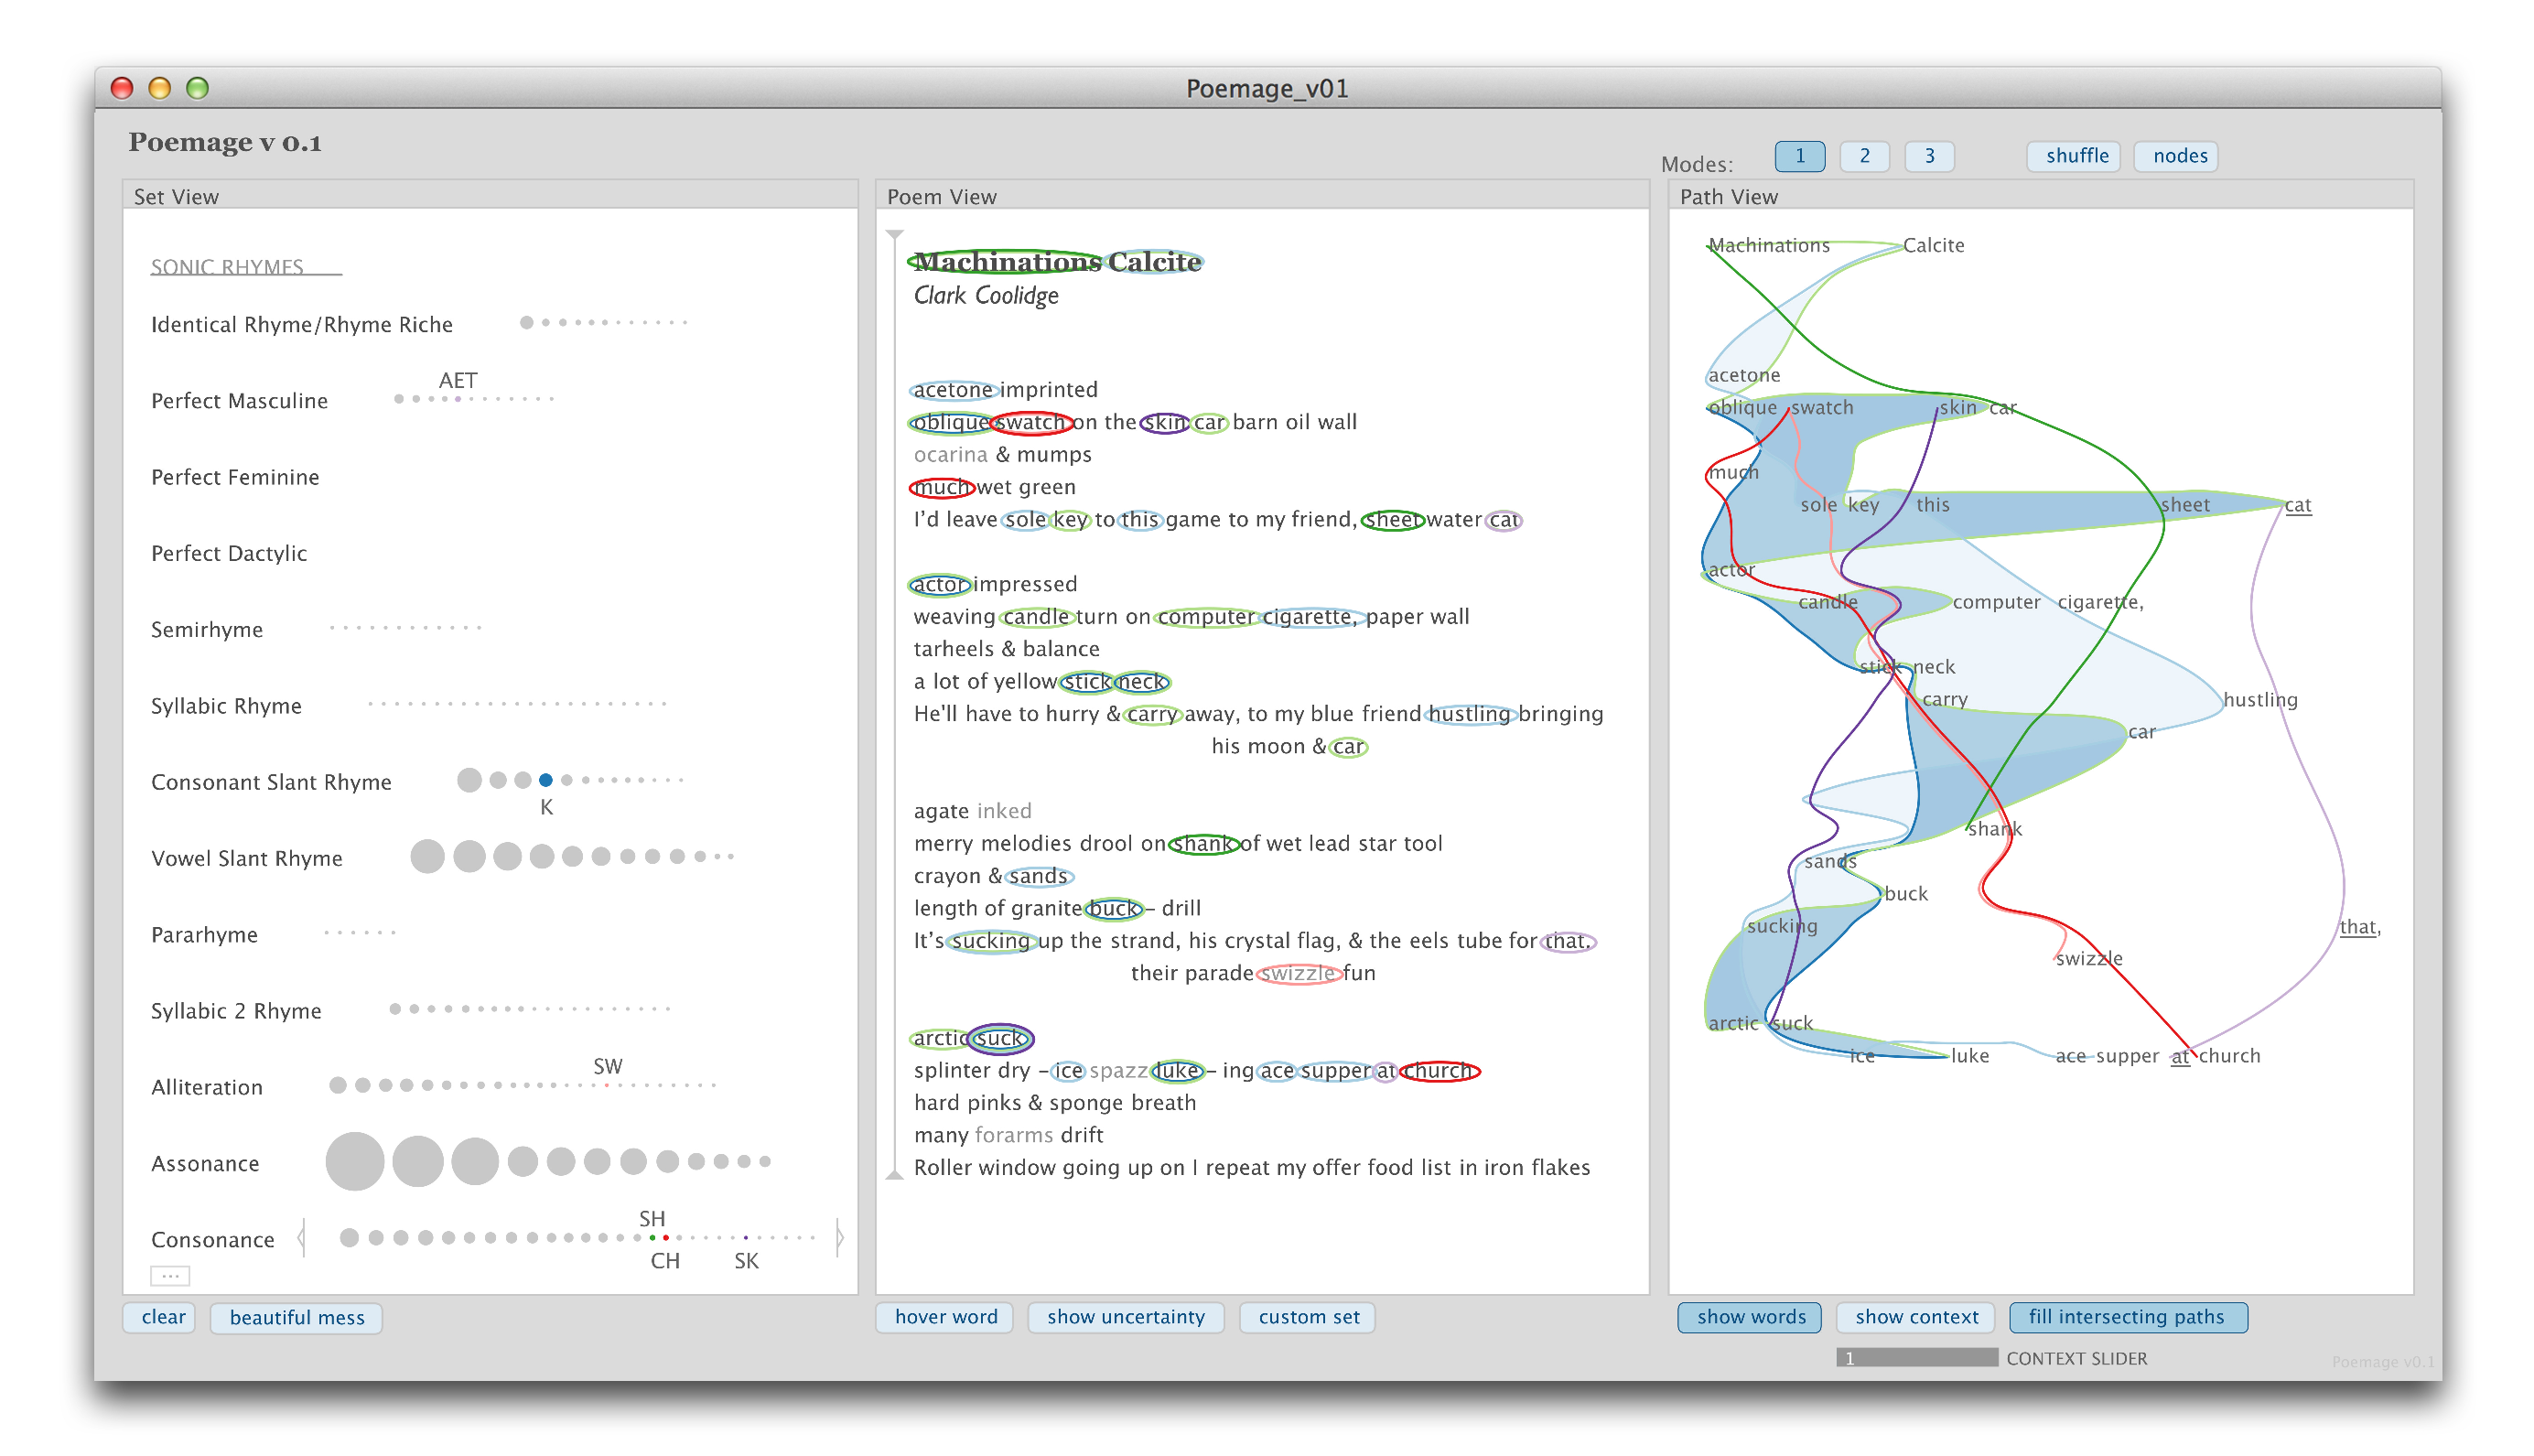
\includegraphics[scale=0.24]{../img/poemage.pdf}
	\caption{An example analysis in Poemage.}\label{screenshotPoemage}
\end{figure}

\subsection*{Ambiances}
This software is unique in the fact that the analysis is integrated in the process of writing. As described in the paper \cite{Meneses2015}, writers input the poem, receive a visualization and can control this visualization with body and hand gestures which in turn influence the poem. By such interconnection the authors aim to make Ambiances a part of the writing process and give it a chance to influence the final result. However, the actual software does not seem to be publicly available.


\section{Generation tools}\label{generation_tools}

Generation of text, especially artistic, is a very challenging task for a machine. As we observed the outputs of exiting tools, we found that the most common flaws include lack of creativity, unnatural and frequent change of the subject, and incoherence. Generation of song lyrics is basically a more specific branch of text generation. Similarly to rhyme detection, it can be distinguished into two main types of methods -- rule-based and machine learning.


\subsection{Rule-based generating}
Rule-based tools are inherently very complex and the output is often limited to certain structure or topic. They usually require the user to input starting configuration, whether it is genre, topic, time period, amount and type of rhymes, phrases, etc. They tend to be less creative but better at rhyming and following the form and structure. To achieve that, they may use rhyming dictionaries (see Section \ref{rhyme_detection_tools}). Simpler ones just use a large set of pre-written templates, e.g. MasterPiece Generator.\footnote{\url{https://www.song-lyrics-generator.org.uk/}} In this thesis, we will focus on generation using machine learning.


\subsection{Generating using machine learning}
The popular approach for generating song lyrics is certainly machine learning in its many forms. It can be proved by the large number of lyrics generators created by enthusiasts, e.g. \textit{These Lyrics Do Not Exist}\footnote{\url{https://theselyricsdonotexist.com/}}, \textit{Freshbots Lyrics Generator}\footnote{\url{https://www.freshbots.org/lyrics-generator}}, \textit{Random Lyrics Generator}\footnote{\url{http://www.anticulture.net/RandomLyrics.php}}, \textit{DeepBeat -- Rap Lyrics Generating AI}\footnote{\url{https://deepbeat.org/}}, \textit{BoredHumans Generator}\footnote{\url{https://boredhumans.com/lyrics_generator.php}}, \textit{RapPad Lyrics Generator}\footnote{\url{https://www.rappad.co/songs-about/}}, and many more. We will further describe Deep-speare (mentioned earlier in Section \ref{ml}) and GPT models, which are considered state-of-the-art in text generation.


\subsubsection*{Deep-speare}
Deep-speare (\cite{lau2018deep}) is a joint neural network architecture that generates only a specific type of poems with strict form and meter -- \gls{sonnet} \gls{quatrain}s. It consists of three models: language model generates one word at a time, pentameter model samples meter-conforming sentences, rhyme model enforces rhyme, and they are all trained together in multi-task learning setting. They present very good results -- generated poems are mostly indistinguishable from human-written ones, apart from expert evaluation, where they report lack of emotion and worse readability.

\subsubsection*{GPT-2}
Generative pre-trained Transformer version 2 (GPT-2) (\cite{radford2019gpt2}) is an unsupervised \gls{transformer_model} capable of various text-processing and generating tasks such as answering questions, translating, summarizing, writing coherent paragraphs, etc. It was created by AI-based research laboratory named OpenAI.

This model was trained on and evaluated against WebText, a dataset consisting of the text contents of 45 million links on sites like Google, Blogspot, GitHub, NYTimes, BBC, eBay, etc. It offers 4 models of different sizes increasing in the number of parameters: 124 million (small), 355 million (medium), 774 million (large), and 1.5 billion (XL) parameter models.

Although this model was only trained for the general task of predicting the next word, given all of the previous words within some text, it can be further fine-tuned for a more specific task to suit user's needs. One example of lyrics generated by fine-tuned GPT-2 is \textit{Keywords To Lyrics}\footnote{\url{https://lyrics.mathigatti.com/}}. However, even without fine-tuning, it can quickly adapt to the style of the input and continue in the same manner, as we show later in Chapter \ref{generation}.


\subsubsection*{GPT-3}
During writing of this thesis, an even larger model GPT-3 (\cite{brown2020gpt3}) with 175 billion parameters was officially introduced. It is considered the largest artificial neural network in May 2020. It was trained on five different corpora: Common Crawl, WebText2, Books1, Books2 and Wikipedia. The architecture is the same as in GPT-2, only number of layers and other parameters increased. It is capable of writing articles indistinguishable from human-written ones (\cite{gpt-3_overview}), even produce functional JavaScript code for natural-language formulated task.

Realizing the power of this tool, the authors did not want to make it available to broad public, fearing it might be misused with bad intentions. Instead they created a form to sign up for access, reviewed individual requests, granting access only to a small portion of them.



\paragraph{}Originally, this thesis intended to focus more on lyrics generation. However, as our research of works in this field shows, there is an abundance of tools for that purpose. Users can just choose a tool that fits their needs. Creating one tool that would be better or more versatile would either require more computing power or literary knowledge, and is above the scope of a master thesis. Therefore, we shifted our main focus to automatic rhyme detection and evaluation, which seems to be far less explored and more interesting topic.



\chapter{Data}

A crucial part of every analysis are the data. To be able to conduct an analysis with results that can reasonably represent the domain, we need to have enough of them - the more the better. 

Our dataset consist of 658,460 song lyrics scraped from the crowd-sourced website 
Genius\footnote{\url{https://genius.com/}}. Sadly, the original author of the dataset is unknown, it has been passed on to us by a colleague as a potentially interesting source for research. However, all song lyrics are publicly available on the Genius website and can be linked with the corresponding item of the dataset via the \textit{url} attribute.


\section{Preprocessing}

In most areas it is very hard to find a dataset of good quality and large quantity. Usually at least one of the two suffers. It is not any different with our data - although the dataset is large, the contents were created by ordinary people and intended for human readers so they are not well suited for automated processing. It is necessary to look closely at the data, remove faulty or redundant items, and clean the rest with preprocessing.

To assess what are the problems in the data and how to address them, we created a very small dataset of only about 10 songs which we cleaned manually. To select these songs, we looked at about 100 random songs and chose the ones that contained the most common faults. We also tried to contain a broad spectrum of errors by focusing on the diversity in the selected dataset. We then iteratively implemented an automated solution for each type of data corruption, comparing the automatically and manually cleaned data, until they matched. We also extracted statistical information that further showed the weak points that needed addressing.

We received the dataset in JSON format, with each song as a separate item, each containing following features:

\begin{itemize}
	\item \textit{title} - the name of the song
	\item \textit{lyrics} - the text of the song's lyrics
	\item \textit{album} - song's album (or null)
	\item \textit{genre} - one of the following: rap, pop, rock, r-b, country
	\item \textit{artist} - song's performer
	\item \textit{url} - the url of the lyrics page on Genius website
	\item \textit{year} - the year the song was produced
	\item \textit{is\_music} - boolean flag distinguishing song lyrics from other texts
	\item other song details: \textit{producer, featured artist, recording location, charts, writer, samples, sampled in, has featured video, has featured annotation}
	\item other website specific information: \textit{rg artist id, rg type, rg tag id, rg song id, rg album id, rg created, has verified callout}	
\end{itemize}

The features from the last two points were \textit{null} for all or most of the items. That, and the fact that they do not give us much more information that would contribute to the lyrics analysis, made them useless and so we decided not to keep them. We removed all songs for which the attribute \textit{is\_music} was False, indicating it was not a song (often a poem or prose) or they did not contain lyrics - 34,259 songs in total. We further removed one song with invalid (incomplete) JSON. After comparing the lyrics to each other, we found and removed 32,551 duplicates.

Upon further inspection, we found out that our dataset also contains lyrics in different languages. We used the neural network model for language identification by Google (CLD3)\footnote{\url{https://github.com/google/cld3}} for the classification. It showed that our dataset contains exactly 100 different languages, most of them represented only marginally. Since other languages did not have enough data to support a good analysis and implementing them would be above the scope of this thesis, we kept only English lyrics. We further removed 832 items with language detection errors. All of them were under 10 lines long so they would not be a valuable addition anyway. At this point our dataset contained 438,037 items.

\begin{figure}[!htb]
	\minipage{0.49\textwidth}
	\includegraphics[width=\linewidth]{../img/histogram_song_length_in_char.png}
	\caption{Histogram of number of characters in songs of our dataset.}\label{hist_chars}
	\endminipage\hfill
	\minipage{0.49\textwidth}
	\includegraphics[width=\linewidth]{../img/histogram_song_length_in_words.png}
	\caption{Histogram of number of words in songs of our dataset.}\label{hist_words}
	\endminipage\hfill
	
\end{figure}
\begin{figure}[!h]\centering
	\minipage{0.49\textwidth}
	\includegraphics[width=\linewidth]{../img/histogram_song_length_in_lines.png}
	\caption{Histogram of number of lines in songs of our dataset.}\label{hist_lines}
	\endminipage\hfill
\end{figure}

To learn more about our data, we created histograms with song's length in characters, words, and lines (see Figures \ref{hist_chars}, \ref{hist_words}, \ref{hist_lines}). Knowing the common issues of extreme values, we manually examined a few of the shortest and a few of the longest items. Confirming our expectations, we found out that they were not valid songs either. The long ones were usually book excerpts or rap improvisation battles, while the short ones were often links to advertisements or motivational quotes. We removed 14 long and 1,838 short lyrics. Although it may not seem as much, it could have strong negative influence mainly during the generation phase. In Figures \ref{hist_chars}, \ref{hist_words}, and \ref{hist_lines}, red lines mark the borders for removal - only the items in between them were kept.


\section{Structure of the data}

This section gives statistical information about the dataset after preprocessing. Table \ref{basic_stats} sums up basic statistics about the data overall and for each genre specifically. Pie chart in Figure \ref{piechart_genres} shows the portions of the data belonging to each genre. All the attributes are listed in Table \ref{stats_nonempty_values}. For some songs, not all attributes are available. Number of items for with non-empty values is given as well.
\begin{table}[h!]
	\centering
	\begin{tabular}{c | r r r} 
		Genre & Songs & Avg. lines per song & Avg. words per line \\ 
		\midrule \midrule
		Pop & 293,679& 36.73 & 5.50\\
		Rap & 99,189 & 64.32 & 6.88 \\
		Rock & 34,372 & 38.73 & 5.30 \\
		R\&B & 5,126 & 52.82 & 5.51 \\
		Country & 3,819 & 38.43 & 5.85 \\
		\midrule
		Total & 436,185 & 43.36 & 5.96 \\
	\end{tabular}
	\caption{Basic statistics about the dataset.}
	\label{basic_stats}
\end{table}



\begin{figure}[h]\centering
	\includegraphics[scale=0.25]{../img/piechart_genres.png}
	\caption{Distribution of genres in the dataset.}\label{piechart_genres}
\end{figure}



\begin{table}[h!]
	\centering
	\begin{tabular}{| c | r |} 
		\hline
		Attribute & Non-empty values \\ [0.5ex] 
		\hline
		lyrics & 436,185 \\
		title & 436,179 \\
		album & 112,060 \\
		genre & 436,185 \\ 
		artist & 436,184 \\ 
		url & 436,185 \\
		year & 96,491 \\ 
		lang & 436,185 \\
		id & 436,185 \\
		word\_count & 436,185 \\
		\hline
	\end{tabular}
	\caption{Attributes and their counts of non-empty values.}
	\label{stats_nonempty_values}
\end{table}

\section{Annotated subset}
From the dataset described above, we separated a subset of 50 songs, 10 song for each genre, and annotated them with rhyme schemes ourselves. We then separated them into a development and test set, so that both groups would have an approximately equal number of non-empty lines per genre (plus or minus 2 lines). We reserved the development set for iterative testing and improvement of our algorithm. The test set was used as an additional checkpoint for final evaluation, as you can read in Chapter \ref{evaluation}.

\section{Chicago Rhyming Poetry Corpus}
For an additional dataset for evaluation, we included one from an outside source -- the Chicago Rhyming Poetry Corpus\footnote{\url{https://github.com/sravanareddy/rhymedata}}, annotated with rhyme schemes by professionals. It contains 1,321 poems from 32 authors written in 14\textsuperscript{th} to 19\textsuperscript{th} century. It has a total of 93,045 lines with an average of 70.44 lines per song. It is the same dataset that was used for training and evaluation of Rhyme Tagger.





\chapter{Rhyme detection}\label{chap-rhyme-analysis}
In this Chapter, we will first consider using available tools for rhyme detection. After not finding the right tool we will reconsider to make the detection ourselves.

Detecting rhymes may seem like a simple task at first, but looking into details one discovers many problems that need to be addressed. As we have seen in Chapter \ref{chap-related-work}, it is not a well-defined task so we need to set the requirements.

Then we progress through individual steps needed to find the rhymes and design a rating that would evaluate song's rhymes:


\begin{enumerate}
	\item phonetic transcription with additional data preprocessing
	\item syllabification and extraction of phonemes after last stressed syllable
	\item comparison of two lines and calculating their rhyme rating
	\item finding all rhymes and assigning a scheme
	\item calculating song rating
\end{enumerate}

\section{Using available tools for detection}
The simplest approach would be to use one of the tools described in section \ref{rhyme_detection_tools}. We want a detector that is free, strong (detects more than perfect rhymes), and offers headless mode (we could run it automatically from code). Ruling out unsuitable tools, we are left with Rhyme Tagger and SPARSAR. Rhyme Tagger is easy-to-use but only outputs rhyme scheme. To be able to automatically evaluate the rhyming quality of a song, we would need more information like stress or rhyme type.

\subsection*{SPARSAR}
SPARSAR, on the other hand, has a very rich and detailed output. Although it is lacking documentation, the \textit{xml} output format is quite descriptive to understand what most of the values represent. It seemed promising so we attempted to pursue this path.

To bridge the outdated system requirements, we contacted the authors for a newer build (for Ubuntu 19.1). They were very helpful and soon we were able to run it on our computer. Nevertheless, we encountered several issues, mostly stemming from the fact that SPARSAR was written in Prolog. Firstly, the xml output was difficult to parse automatically, as the values were written in Prolog syntax, using the same delimiter for different levels of separation. Secondly, SPARSAR parses the text in sentences but lyrics are usually written without punctuation. We added punctuation using \textit{punctuator2} (\cite{tilk2016punctuation}) which also added space for error. 

Lastly, when SPARSAR encountered an unknown word, it failed for the entire song. Since our data were crowd-sourced, it contained many unusual words, so in the beginning it failed on 80\% of our data. We iteratively worked with the authors for months on fixing bugs and adding words (mainly contractions, such as I'mma, y'all, yo', 'em, etc.) into their dictionary. In the end, we were able to successfully run it on 95\% of our data.

However, we were still not very satisfied with the result. As you can see in the example in Table \ref{sparsar_wrong_scheme}, it failed to detect the perfect rhyme between 2\textsuperscript{nd} and 4\textsuperscript{th} line, and instead marked a rhyme on line 1 and 3, where there was none. The example shows the first four lines of the song, but the scheme letter \textit{h} does repeat only once more on line 34. Such errors were not sparse and led us to believe that the encoded inclination of this tool to look for sonnet-shaped schemes caused it to make errors in the diverse schemes of song lyrics. It may be a great tool for sonnets, but we have found it insufficient for our purpose, so we proceeded to create our own rhyme detector.


% \begin{table}[h!]
% 	\centering
% 	\begin{tabular}{c c c} 
% 		Scheme & Line & \begin{tabular}{@{}c@{}}Last word's pronunciation \\ (as assigned by SPARSAR)\end{tabular}  \\ [0.5ex] 
% 		\midrule
% 		a & Pulled out from the station & s-t-ey-sh-ah-n \\ 
% 		h & fifteen after two & t-uw \\
% 		a &	300 miles away from Vegas & v-ey-g-ah-s\\
% 		b & We had nothin better to do & d-uw\\
% 	\end{tabular}
% 	\caption{Exampleof incorrect scheme assignment by SPARSAR. Excerpt from the song \textit{Good Life}.}
% 	\label{sparsar_wrong_scheme}
% \end{table}

\begin{table}[h!]
	\centering
	\begin{tabular}{@{}c c c c@{}}\toprule
		\multicolumn{2}{c}{Scheme} & Line & Last word's pronunciation \\\cmidrule{1-2}
 		correct & SPARSAR & & as assigned by SPARSAR  \\
		\midrule
		A & a & Pulled out from the station & s-t-ey-sh-ah-n \\ 
		B & h & fifteen after two & t-uw \\
		C & a &	300 miles away from Vegas & v-ey-g-ah-s\\
		B & b & We had nothin better to do & d-uw\\
		\bottomrule
	\end{tabular}
	\caption[Example of incorrect scheme assignment by SPARSAR. Excerpt from the song \textit{Good Life}]{Example of incorrect scheme assignment by SPARSAR. Excerpt if the beginning of the song \textit{Good Life}. The correct scheme is marked in capital letters,	the scheme assigned by SPARSAR is marked in lowercase letters. }
\label{sparsar_wrong_scheme}
\end{table}


\section{Defining the requirements}\label{defining_the_requirements}
Before we dive into algorithm selection and implementation details of our detector, let's define what exactly do we want our detector to do. Additionally, we also establish terms for common cases in Table \ref{terms}, to keep our further explanations short and clear.
\begin{table}[h!]
	\centering
	\begin{tabular}{>{\bfseries}l l} 
		component & a vowel or a consonant cluster in a syllable\\
		rhyme candidates & two lines that are being compared for rhyme \\
		rhyming fellows & two lines that rhyme together\\
		rhyming part & the exact components that participate in rhyme \\&(i.e. are equal or similar in sound)\\
		rhyme group & a group of lines that all rhyme together\\& (i.e. have identical scheme letter) \\
		rhyme rating & rating of the quality of one rhyme between two lines\\
		song rating & rating of the rhyming quality of the entire song\\
	\end{tabular}
	\caption{Establishing terms.}
	\label{terms}
\end{table}

\paragraph{Input}
Although we realize sound can affect rhymes, for the purpose of this thesis we will focus solely on text. As \cite{rhymes_overview} points out, most works focus on rhyme schemes in well structured poetry instead of common rhymes in text. We do not have standard rhyme scheme patterns nor fixed syllable counts -- song authors use rhymes arbitrarily. Although in some genres, mainly rap, rhymes in the middle of the line (\gls{internal_rhyme}s) can occur, as we decided in Chapter \ref{chap-related-work} we will only focus on \gls{end_rhyme}s in this thesis. For our input, we expect song lyrics in English, formatted in lines with rhyme always at the end of line. Optional empty lines between stanzas or chorus will be preserved but skipped.

\paragraph{Output}
The main element of our output is rhyme scheme. As a single element, it gives the best overview of the song and more importantly, it allows us to compare our detector with others or with the \gls{gold_data}. Additionally, we want more information to assess rhyme quality: rhyme rating for each individual rhyme, song rating, rhyme type, pronunciation of the rhyming part, optional modification of stress, etc.


\section{Pronunciation}
\subsection{Phonetic alphabets overview}
Unlike many other languages, English does not have a straightforward pronunciation rules. Therefore to be able to assess rhymes, we need to transcribe our text into a phonetic alphabet first. There are two commonly used alphabets to choose from -- IPA and ARPAbet. The original International Phonetic Alphabet (IPA) used since 1888 uses one UNICODE character to encode each phoneme and it is commonly used for example in dictionaries. Since it uses non-ASCII characters, ARPAbet was developed as an equivalent for computers. It has two versions: 1-character that uses upper-case and lower-case letters and (the more common) 2-character version where each phoneme is represented by one or more upper-case ASCII characters (\cite{lea1980trends})(see Table \ref{pronunciation_table} for comparison). We will be using the 2-character ARPAbet because it is used by the CMUdict.

\begin{table}[h!]
	\centering
	\begin{tabular}{c c c c} 
		Example word & IPA & 1-character ARPAbet & 2-character ARPAbet \\ [0.5ex] 
		\hline
		st\textbf{o}ry & \textipa{O} & c & AO \\ 
		bu\textbf{tt}er & \textipa{R} & F & DX \\
	\end{tabular}
	\caption{Short comparison of different pronunciation alphabets.}
	\label{pronunciation_table}
\end{table}
\subsection{CMUdict}\label{cmudict}
Carnegie Mellon University Pronouncing Dictionary (CMUdict) is an open-source pronunciation dictionary.\footnote{\url{http://www.speech.cs.cmu.edu/cgi-bin/cmudict}} Currently it contains 134,373 words (including their inflections) and their pronunciations in 2-character ARPAbet. 
For each word, there is one or several possible pronunciations in North American English including stress markers for primary, secondary or no stress. For the implementation, we used its Python wrapper package \textit{cmudict}.\footnote{\url{https://pypi.org/project/cmudict/}} To use this we had to strip the input of punctuation and convert it to lower case.

CMUdict is a large dictionary and it includes also slang words so it should cover most of our input. To test this, we looked at all last words on each line of our data (since those are the important ones for rhyme analysis) and we found out that 5.52\% of them are not included in CMU dictionary. We manually inspected a small portion of them and found out that they can be mostly split into the following 5 categories:

\begin{itemize}
	\item uncommon words, e.g. superglue, redundantly
	\item misspelled words, e.g. decsion, girlfren
	\item numbers
	\item foreign words, e.g. revoluccion, ecolli
	\item interjections and onomatopoeia, e.g. shoooshooo, woahwoah
\end{itemize}

\subsection{Dealing with out-of-dictionary words}
In an attempt to decrease the amount of out-of-dictionary words, we replaced the closing single quotation mark ``\textipa{’}'' (U+2019) with the typewriter apostrophe ``\texttt{\fontencoding{OT1}\selectfont\symbol{13}}''
 (U+0027) since only the second variant of apostrophe is accepted by CMUdict. However, this only decreased the percentage of unrecognized words to 5.47\%.

Clearly, we needed a way to estimate the pronunciation for the rest of the words, so we used grapheme-to-phoneme library \textit{g2p} by \cite{g2pE2019}. It predicts the pronunciation for out-of-dictionary words using deep learning seq2seq model by TensorFlow (\cite{tensorflow2015-whitepaper}).

Even having the pronunciation for every word will not ensure we find every rhyme intended. Song artists may take their liberty in modifying or skewing the pronunciation to make the rhyme work. Sometimes they can also sing two syllables in one beat or use an unusual pronunciation from different culture to convey a message. As we established in the beginning, we will focus only on information retrievable from the text and ignore these possible deviations in pronunciation.

\section{Syllabification}
\subsection{Alignment}
When comparing lines for rhymes, we have to establish a system of alignment so that we analyze only relevant pairs of phonemes. Initially, we created a simple rhyme detector that just traversed both verses backwards phoneme by phoneme\footnote{For simplification, we use the term phoneme for one symbol in ARPAbet.} and compared them. However, rhyming words do not have to have an equal number of phonemes. For example words in the Table \ref{phon_misalign_table} have a 2-syllable rhyme. If we compared all phonemes one by one they get misaligned on consonant clusters S-T-R and P-L and we will miss the penultimate syllable rhyme. For forced rhymes this inherently becomes a very frequent issue.

\begin{table}[h!]
		\centering
	\begin{tabular}{c r} 
		Word & ARPAbet transcription \\ [0.5ex] 
		\hline
		constrain & K AH N -- S \space\space T R EY N \\ 
		complain & K AH\space  M --  P L EY N \\
	\end{tabular}
	\caption{Example of misalignment when aligning by phonemes.}
	\label{phon_misalign_table}
\end{table}

We need to make sure that we are comparing corresponding parts of verses otherwise we will miss the rhyme. A better approach would be to compare corresponding syllables because they naturally create an alignment in the rhythm of the song. Each syllable can be further split into 3 groups (``CVC'') -- leading consonant cluster (\textit{onset}), vowel (\textit{nucleus}), and trailing consonant cluster (\textit{coda}). Consonant clusters can sometimes be empty. For syllabification we used Python library \textit{syllabify},\footnote{\url{https://github.com/kylebgorman/syllabify}} which requires input in ARPAbet (we use the output of CMUdict) and conveniently returns syllables in CVC triplets as described above.


\subsection{Extracting relevant components}\label{extracting_relevant_phonemes}
Since we established that rhymes are located at the end of each line, there is no need to analyze the entire verse. How far should we look? The first choice would be to look at the last word only. However rhymes can extend over more words as we see in example in Figure \ref{two-word_rhyme}.
\begin{figure}[htb]\centering
	I was the man the Duke \textbf{spoke to};\\
	I helped the Duchess to cast off his \textbf{yoke, too};\\
	\caption{An example of two-word rhyme from \textit{The Flight of the Duchess} by Robert Browning.} 
	\label{two-word_rhyme}
\end{figure} 

When we look at rhyme types, they do not go further then the first stressed syllable (looking at the line backwards). Notably, even if the rhyme does extend further we can ignore the rest because it cannot increase the rating. For example, if there are more rhyming syllables preceding the perfect rhyme, they cannot make the score better. Similarly, if the rhyme is not perfect, syllables preceding the final stress would already be considered an \gls{internal_rhyme} -- which is also used (mainly in rap lyrics) but less valued than the classical end rhyme and as stated in Section \ref{defining_the_requirements}, not a target of analysis in this thesis. We will therefore limit our window to the minimal number of syllables needed to include the stressed syllable in both rhyme fellows. If one rhyme fellow needs less syllables than the other (i.e. it is an imperfect rhyme), we will move stress to the right to match the shorter syllable span (and later decrease the rhyme rating by a \textit{stress penalty, cf. Section~\ref{rhyme-rating}}).


\section{Rhyme analysis}
\subsection{Finding similar phonemes}
Finding perfect rhymes is easy -- phonemes after the last stress need to agree exactly. Imperfect rhymes can be found similarly, using the trick of moving the stress described in Section \ref{extracting_relevant_phonemes}.
To set ourselves apart from simple rhyme detectors, we need to detect more than just perfect and imperfect rhymes -- we need to find forced rhymes as well. To determine forced rhymes we have to assess the match in sound of individual phonemes.

For this, we took inspiration from \cite{plechavc2018collocation}. He used the fact that rhymes tend to reoccur and, having enough data, commonly co-occurring pairs are most probably rhymes even without the knowledge of their pronunciation. He calculated the probabilities of phoneme co-occurrences in line-end words from their frequencies in data, used this co-occurrence matrix to predict rhymes, and then iteratively recalculated the matrix using the EM algorithm.

However, our system of alignment is different so our matrix components will look differently. The differences are shown in Table \ref{alignment}. The first difference is that Plecháč only uses vowels and consonant clusters without acknowledging the syllable separation. We do separate the consonant cluster into two on the border of syllables (e.g. ``rp`` in carpenter is in one cluster for Plecháč, but in two separate clusters for us). The second difference is that Plecháč recognized the position of the component and paired only the components on the same position (i.e. both ``\textipa{@}'' in carpenter are in separate groups because they occur on different positions in the word). We do not believe that position has an effect on phoneme similarity and therefore we add it together for all positions, e.g. if once two phonemes co-occur on 3\textsuperscript{rd} position and once on the 5\textsuperscript{th} we will say that this pair of phonemes has 2 co-occurrences.

\begin{table}[h!]
	\centering
	\begin{tabular}{c r} 
		Plecháč & \textipa{\color{blue}k \color{magenta}A: \color{PineGreen} r.p \space\space \color{BurntOrange} @ \color{BrickRed}  n.t \space\space\color{Cerulean} @ \color{Fuchsia}r}\\
		Us & \textipa{\color{blue}k \color{magenta} A: \color{blue}r \space .p \color{magenta} @ \color{blue} n \space .t \color{magenta} @ \color{blue}r} \\
	\end{tabular}
	\caption[Comparison of alignments]{Comparison of our components for word \textit{carpenter} with those of \cite{plechavc2018collocation}. Different color signifies different component group.} 
	\label{alignment}
\end{table}

Another difference is that Plecháč only looks at the last word and its 1 or 2 last syllables while we look at everything after the last stress up to 4 syllables.

Knowing that perfect match in sound always means perfect rhyme (which should intuitivelly get the highest possible rhyme rating of 1.0), we froze the values on matrix diagonal to reflect it. In \cite{plechavc2018collocation}, the diagonal was being recalculated as the rest of the matrix, and although it seemed to converge to high numbers we felt it did not reflect the superiority of the perfect match.

To calculate the probabilities in the matrix, we used the formula from \cite{plechavc2018collocation} adding the adjustments described above. The formula for a the value in the matrix on coordinates i, j is as follows: 


	    \[ p(i,j) = \begin{cases} 
	    \mbox{1.0,} & \mbox{if  i=j} \\ 
	  \dfrac{f(i,j)}{f(i,j) + f(i)f(j)},
	     & \mbox{otherwise} \\
	    \end{cases} \]

where\textit{ f(i,j)} represents the frequency of the co-occurrence of the pair of components \textit{i} and \textit{j}, and similarly \textit{f(i)} represents the total number of occurrences of the component \textit{i}.
\MP{Ale Plecháč definuje f(i,j) jako \textbf{relative} frequency, tedy pravděpodobnost souvýskytu, nikoli absolutní počet souvýskytů.
Obdobně f(i) = count(i) / total\_count. Kde $\sum_i f(i) = total\_count$.
Je-li to jen nepřesnost v textu, tak jen doplňte k frequency přívlastek relative a nahraďte ten total number of occurrences.
Je-li v kódu taky absolutní počet, tak nevím -- opravit to už zjevně není čas.
Omlouvám se, že jsem si toho všiml až teď.
}
\MP{Ještě by chtělo lépe definovat, co je occurrence -- tedy výskyt dané komponenty na konci řádku po posledním přízvuku.
Započítáváte do toho i výskyty, kde odpovídající komponenta v rhyming fellow je identická?}
\MP{I ty co-occurerences by bylo dobré lépe definovat -- je to souvýskyt na odpovídají pozici v rhyming fellow, přičemž je k tomu tedy potřeba mít nějak určené rýmy,
abychom věděli, který z předchozích řádků je ten fellow, což máte vysvětlené v následující sekci.}

Technically, the matrix is only triangular because the order of \textit{i} and \textit{j} does not matter.

\subsection{Training the detector} \label{analysis:training}
What we have just described is basically step 3 of learning the matrix using the EM algorithm. The whole outline can be summed up in 4 steps:
\begin{enumerate}
	\item Initialize the matrix of vertical collocation probabilities.
	\item Find rhymes using this matrix.
	\item Adjust the matrix based on detected rhymes.
	\item Repeat steps 2 and 3 until convergence.
\end{enumerate} 

To improve the matrix in step 3, in each iteration we will count the vertical collocations only from the pairs that were marked as rhyming in the previous iteration.


For the matrix initialization, Plecháč calculates the vertical collocations in the data and preserves only pairs with number of vertical collocations above a set threshold. We instead initialized it with the default value of 0.2. 

Finding rhymes (step 2) is further described in Section \ref{finding-all-rhymes}.


\subsection{Rhyme rating}\label{rhyme-rating}
 We will first calculate rhyme ratings for pairs of verses and then use them to calculate an overall song rating. Not only do these rhyme ratings help us evaluate the rhyming quality of the song but they might also be an interesting feedback for the users (e.g. authors of song lyrics) -- we thus show the rhyme ratings in our web visualization as described in Section~\ref{visualization-matrix}.
 
 
 For each rhyme, we would like to assign a rating between 0 and 1. Since perfect rhyme is often in literature described as superior because it represents the perfect match in sound it will logically receive the highest rating of 1.
 
 For other cases, such as imperfect rhymes or some forced rhymes, where it was necessary to move the stress to the rhyming part, we will give a penalty of -0.1 for moving the stress. This includes both the case when stress on one line had to be moved to match the other, and the case when stress on both lines had to be moved to exclude non rhyming syllables from the rhyme.
  
	When the phoneme sounds are similar, we will assign rhyme rating as a simple multiplication of probabilities for the individual components from the matrix. 

This is the final formula
	
	\[rhyme\ rating = stress\_penalty + \prod_{i,j\ \epsilon\ rhyming\ part} p(i,j) \]
	
where \textit{stress\_penalty} is 0 if stress was not moved, -0.1 otherwise. Indices \textit{i, j} iterate over components in rhyming parts of the both words.





\section{Scheme}
\subsection{Finding all rhymes}\label{finding-all-rhymes}
To search for rhymes in the full lyrics, we need to decide which verse pairs to check. The most straight-forward approach would be ``brute force'' -- try each line with all the other lines. Besides its obvious disadvantage of increased time requirements it also detects rhymes that span across tens of lines. It is not strictly defined how many lines apart can the rhyme fellows be to still be considered a rhyme -- the author can even make it a part of his artistic expression, e.g. in \textit{Author's Prologue} by \cite{thomas1952author} the 1\textsuperscript{st} line rhymes with 102\textsuperscript{th}, 2\textsuperscript{nd} with 101\textsuperscript{th} and so on. Realistically, a rhyme between a line in the beginning of the lyrics and 20 lines later, would hardly be noticed at all by song's listeners -- it requires a close proximity of rhyme fellows within the poem. We decided to set the default window size to 5, to include support for rhyme propagation within stanzas.


We traversed the song lyrics from beginning to the end, line by line, for each line trying all rhyme candidates in the given window.

Some words may have multiple possible pronunciations -- in that case we evaluate each possible combination of pronunciations for all words in the given pair. For every such combination we assign rhyme rating and create a list of candidates.

As \cite{rhymes_overview} states, it is difficult to know where to draw the line between intended rhyme and accidental word similarity. However, a threshold must be set to draw a boundary between the two. By default, we have set this threshold to 0.8 because we found it to work quite well in our data. However, it can be adjusted by users to their value of choice; similarly with other parameters such as window size. The list of rhyme candidates can now be reduced to the ones with rhyme rating above the selected threshold.

From this list of candidates for each line, we select only the candidate with the highest rhyme rating. When the ratings are identical, we select the closest line. Other candidates are saved, in case changes need to be made later in scheme adjustment phase, cf. Section~\ref{sec:scheme-adjustment}. When the line does not have any suitable rhyme candidates, it is assigned rating 0. If the line rhymes with a candidate that is already a part of a rhyme, they join together into a rhyme group of 3 (or more) lines.
 



\subsection{Assigning rhyme scheme}\label{sec:scheme}
 Rhymes in songs or poems are typically marked using a rhyme scheme. That means each verse gets assigned a letter -- lines that share the same letter rhyme and those with different letters do not. We also decided to adapt this common notation. In case the song needs more letters than there are in the alphabet, we will add another letter and continue alphabetically -- a, b, c, ..., aa, ab, ac, ..., ba, bb, bc, ..., ca, etc.
 
 There are two options for representing non-rhyming lines. The first is to assign every non-rhyming line the same default character. We chose this option as the default (using character ``--''), because it is easier to read for the user. The second option is to assign each non-rhyming line a unique rhyme scheme letter. This approach is more suitable for metrics that look at rhyme scheme letters as clusters of rhyming words. We support both options and can convert one into the other when needed.

\subsection{Scheme adjustment}\label{sec:scheme-adjustment}
In some cases, the algorithm of selecting the best rhyme for each line does not yield the best possible scheme. Consider, for illustration, the example in Table \ref{scheme_adjustment}. There is a perfect rhyme between lines 1-2 and 3-4, and a forced rhyme between lines 2-3. With the algorithm as is, it would receive the \textit{aaaa} scheme. However, that is not what a human, for example a gold data annotator, would assign. He would see that similarity inside the first and the second tuple is greater so they logically form two rhyme groups and the scheme is \textit{aabb}. 

Additionally, song rating (as defined in the following section~\ref{sec:song-rating}) for scheme \textit{aaaa} would be less than 1 (because of the lower rating of the forced rhyme between lines 2 and 3) while the song rating for \textit{aabb} would be equal to 1. Loosing rating by marking weaker rhymes does not make sense, so we must add an exception to only keep the better score. We can see that this problem is similar to the problem of maximizing song rating. 

\begin{table}
	\begin{tabular}{l l}
		1&Packs of Backwoods and Dutches, leave the Swishers for the \textbf{sweeties}  \\
		2&Only roaches in the dishes we be ripping up your \textbf{beedies}  \\
		3&We be ripping up your treaties, I ain't ripping if it's \textbf{seedy}  \\
		4&I ain't riffing, I ain't raffing, I'm just rapping on a \textbf{CD} \\
	\end{tabular}
	\caption[Scheme adjustment example.]{Example of scheme adjustment from \textit{aaaa} to \textit{aabb}. Excerpt from the song \textit{Whooping Cough} from  our dataset.}
	\label{scheme_adjustment}
\end{table}

To address this issue, we have to do one more iteration over the resulting rhyme groups. We focused only on rhyme groups of size 4 and larger because for smaller group such changes would not increase the score. For a larger group, we iterate over the rhymes, starting from the ones with the lowest rating, and try how would removing this rhyme affect the song rating. If it increased the song rating, we keep the change and split the rhyme group as necessary. If the rating did not increase, we try removing the next rhyme, and if we ran out of rhymes to remove, we keep the group as is.

\section{Calculating song rating}\label{sec:song-rating}
The next step is to combine these rhyme ratings into one final rating for the entire song. We will use the straight-forward approach of averaging the assigned rhyme ratings. The dilemma here is where to store the rhyme rating since rhyme is a property of two lines. The first logical idea would be to store it with each line participating in the rhyme. However, then we would add it to the final song rating twice. Moreover, for larger rhyme groups, it would be disproportionate, because third and all the following lines would be added only once. 

Therefore, we decided to store the rating only with the second line of the rhyme. That means the first line in each rhyme group will always be assigned the default value ``-''. It cannot be assigned rhyme rating 0 because that would mean it is a non-rhyming line and would lower the final average. In summary, song rating is the average of rhyme ratings for all rhymes except the lines with unassigned rating ``-''.

\chapter{Evaluation}\label{evaluation}
In this chapter, we will evaluate our rhyme detector. In the beginning, we will compare its performance with Rhyme Tagger. Then we will use it to analyze our dataset and calculate statistics about song lyrics.

\section{Performance evaluation on schemes}
\todo[inline]{Popisat preco nejdu reddy data su menej vhodne na moju detekciu rymov}

\section{Statistical analysis of the dataset}
Although our detector was trained on our dataset, it was unsupervised so we can still use our detector to evaluate this dataset and give us new statistical information about a large number of song lyrics. We ran rhyme detection for nearly half a million songs and summed up the results in Tables \ref{rhyme_line_stats}, \ref{rhyme_types_perc}, \ref{rhyme_group_size}, \ref{song_rating_stats}, and \ref{rhyme_stats}. In the rest of this section, we will look at them more closely and discuss the outcome that might be surprising, or the opposite, confirms the specific  characteristics of a particular genre. Extreme values are emphasized in the tables. Keep in mind, that the lyrics and their classification to genres is crowd-sourced and might be biased.
\begin{table}[h!]
	\centering
	\begin{tabular}{l | r r r r r} 	
		Genre & 			Pop & 		Rap & 		Rock & 		R\&B & 		Country\\ 
		\midrule
		 Total songs& 293,679 & 99,185& 34,372& 5,125& 3,816 \\
		Total lines& 9,104,273 &5,661,603& 1,087,245& 225,344& 121,207 \\ 
		Total rhyming lines& 4,536,554& 2,849,905& 523,879& 117,862& 61,142 \\ 
		 Rhyming lines (\%) & 49.8\%& 50.3\%& 48.2\%& 52.3\%& 50.4\%  \\
		 Average lines per song & 31.001 & \textbf{57.081} & 31.632 & 43.970 & 31.763  \\

	\end{tabular}
	\caption{General statistics about dataset and rhymes, per genre.} 
	\label{rhyme_line_stats}
\end{table}

In Table \ref{rhyme_line_stats}, we sum up the basic information for all genres including the portion of lines that rhyme and we can already see some interesting results. Surprisingly, the highest portion of rhyming lines is in the R\&B genre. We do not see any characteristic of this genre that could cause this. However, it is not a big difference and maybe having more examples from this genre would make it less significant. 

We can see that throughout genres typically only about half of the lines rhyme. This shows, that rhyming in songs is not as essential as perhaps in poems. Predictably, rap has a significantly higher average number of lines per song which confirms the fact that this genre is more talkative. What may be unexpected is that it is nearly two times more than for the other genres -- only R\&B slightly stands out but that is not a surprise because it has been influenced by rap.

\begin{table}[h!]
	\centering
	\begin{tabular}{l | r r r r r} 	
		Genre & 			Pop & 		Rap & 		Rock & 		R\&B & 		Country\\ 
		\midrule
		Perfect masculine &	72.5& 	\textbf{58.2}& 	72.3& 	70.2& 	73.5 \\
		Perfect feminine &	7.9&		8.4& 		7.7& 		8.5& 		6.2 \\
		Perfect dactylic & 	0.7 &		0.5 & 	0.9 &		0.5& 		0.3 \\  
		Imperfect & 		12.0& 	\textbf{22.3} & 	12.1 & 	13.5 & 	12.2 \\
		Forced &  			6.9 & 	\textbf{10.6} & 	7.0 & 	7.3 &		7.8 \\
	\end{tabular}
	\caption{Percentage of different rhyme types from all rhymes in the dataset, per genre.} 
	\label{rhyme_types_perc}
\end{table}

Next, Table \ref{rhyme_types_perc} shows distribution of different rhyme types. It did not come as a surprise that the most common type, by a long shot, is perfect masculine. The reasons behind this might be several -- not only has perfect match the strongest effect melodically, it is also the easiest to come up with, and makes the lyrics easy to remember. The multi-syllable perfect rhymes have a lower percentage as longer matching word pairs are rather rare. The amount of forced rhymes might be higher in reality because their detection is the hardest and they might be missed more often.

Concerning rhyme types, we see that genres are generally not very different, except for rap. Rap is very unique with rhymes, its artists are known for playing with them more creatively, using \gls{internal_rhyme}s, consonance, and assonance more often. They frequently play with emphasis what can be seen as a rapid increase in imperfect rhymes. There are more forced rhymes as well and perfect rhymes are decreased as a result.

\begin{table}[h!]
	\centering
	\begin{tabular}{l | r r r r r} 	
		Genre & 			Pop & 		Rap & 		Rock & 		R\&B & 		Country\\ 
		\midrule
		2-syllable rhymes & 91.1& 90.3& 91.1& 90.6 & 93.3\\
		5-syllable rhymes& 8.2& 9.2& 8.0& 8.9& 6.4  \\
		8-syllable rhymes& 0.7& 0.5& 0.9& 0.5& 0.3 \\
		Perfect sound match & 93.1&\textbf{ 89.4}& 93.0& 92.7& 92.2  \\
		Stress moved & 14.5& \textbf{28.3}& 14.5& 16.5& 14.8 \\
		
	\end{tabular}
	\caption{Statistics about rhyme properties in general, disregarding rhyme types, in percentage from total rhymes.} 
	\label{rhyme_stats}
\end{table}

Table \ref{rhyme_stats} is quite similar to the previous table, but by counting syllables regardless of rhyme type, and evaluating sound match and stress separately, it offers us a little bit different angle. By seeing that the percentages of 8-syllable rhymes match the percentages we have seen in Table \ref{rhyme_types_perc}, we can assume that 8-syllable rhymes might be exclusively perfect. The decreased match in sound and increased moving of stress in rap confirm the unique properties of rap we have seen previously.

A slightly increased percentage of 2-syllable in country may be noteworthy but we see no significant properties of country that could support this as a general claim.

\begin{table}[h!]
	\centering
	\begin{tabular}{l | r r r r r} 	
		Genre & 			Pop & 		Rap & 		Rock & 		R\&B & 		Country\\ 
		\midrule
		Average groups per song& 6.134 &\textbf{11.484} &6.091 &8.620 &6.676  \\
		Average groups per 100 lines &19.787 &20.119 &19.255 &19.605 &\textbf{21.018} \\
		Max groups per song & 169 &224 & 81 & 48 &98\\
		Average group size & 2.518 &2.502 &2.502 &2.668 &\textbf{2.400} \\
		Max group size & 159 &98 & 68 & 42 & 24\\
	\end{tabular}
	\caption{Statistics about rhyme group size per genre.} 
	\label{rhyme_group_size}
\end{table}

Table \ref{rhyme_group_size} summarizes statistics concerning size of rhyme groups. We can observe nearly double average size for rap compared to other genres, which directly corresponds to nearly double average song length, as we have seen in Table \ref{basic_stats}. 

An interesting observation can be made for country -- average number of rhyme groups per 100 lines is slightly higher than for other genres. This corresponds with average group size being lower -- obviously country tends to contain more and smaller rhymes groups. It would be interesting to know, whether this is only a property of our dataset or a property of country music in general. Although maximum group size does not tell us any general information about the group because it may only be an outlier, but it is still interesting to see, that this number is again the smallest for country.

\begin{table}[h!]
	\centering
	\begin{tabular}{l | r r r r r} 	
		Genre & 			Pop & 		Rap & 		Rock & 		R\&B & 		Country\\ 
		\midrule
		Average song rating& 0.432 & \textbf{0.599} &0.420 &0.520 &0.456  \\
		Median & \textbf{0.521} & 0.380 &0.357 &0.235 & 0.269\\
	\end{tabular}
	\caption{Song rating per genre.} 
	\label{song_rating_stats}
\end{table}

Looking at average and median ratings in Table \ref{song_rating_stats}, we can observe two curious extremes -- rap having the highest average rating and pop with the highest median rating. Rap leading in the average, but this dominance not being translated into median, tells us that there must be some extremely high rated songs that pulled up the average. Although we did not predict this result, it shows that some artists probably took the importance of rhyme in rap very seriously and elaborately incorporated it densely into their lyrics.

Highest median in pop shows that many pop songs are filled with more rhymes what can be explained by their strong tendency to be memorable. However, it seems that there are some low extremes that pulled the average rating down.
\chapter{Visualization}
To make the results more approachable for a common user, it is always better to visualize them in some way. Therefore, to demonstrate our detector's capabilities, we created a website that visualizes rhymes and their quality, shows statistics, and allows user to experiment with the parameters. This way, it can be used by anyone without any programming background.

\section{Input}
The input page consists of a text-box for song lyrics, a card with parameters, and an \textit{Analyze} button, as seen in Figure \ref{web-form}.

The text-box expects text input of song lyrics, separated into verses with newlines such that rhymes are at the end of the line. Once text is entered, \textit{Analyze} button will be enabled.

For analysis, the default parameters are pre-filled, but user can choose to change them. Selecting the checkbox \textit{Perfect rhymes only} will trigger the detector to only detect perfect rhymes. Changing the size of the window will affect how many lines apart can rhyme be. Smaller window is better for creating rhyme schemes, while longer window (e.g. equal to song length) will give better overview of rhyme repetition throughout the entire song and give a more interesting matrix visualization. \textit{Rhyme threshold} parameter sets the minimal rhyme rating -- rhymes with lower rating will be discarded.

Pressing the \textit{Analyze} button will start the analysis and minimize the input page. For the duration of rhyme detection, loader is shown to inform the user their request is being processed. When the back-end returns the results, analyze page is expanded to show the visualizations. If desired, user can expand input page, edit the input, and re-submit for analysis.

\begin{figure}[h]\centering
	\includegraphics[scale=0.3]{../img/web-empty-form.png}
	\caption{Website's form for entering the lyrics and setting the parameters.}
	\label{web-form}
\end{figure}

\section{Visualization of the results}
Visualization page contains lyrics with scheme, matrix visualization of rhymes, and short statistics. It is primarily designed for songs of short or moderate length, longer lyrics may not fit on the screen with the analysis side-by-side, and will have to be rearranged in a column, which makes the results less comfortable to read.

\subsection{Lyrics and statistics}
Lyrics with their assigned scheme letters and line number are shown on the left, as we can see in Figure \ref{web-analysis_window5}. Rhyming lines are highlighted, each with a color corresponding to its rhyme type. For the sub-types of perfect rhyme, we selected similar colors to indicate that they are more closely related -- namely red for \textit{masculine}, orange for \textit{feminine}, and yellow for \textit{dactylic} rhymes. \textit{Imperfect} rhymes are highlighted in blue and \textit{forced} in green color. When user hovers over a rhyming line, this line and all lines rhyming with it are highlighted.

Statistics is shown on the right under the matrix. It contains song rating and percentages of different rhyme types in the song.

\begin{figure}[h]\centering
%	\includegraphics[scale=0.24]{../img/web-empty-form.png}
	\caption{Screenshot from analysis.}
	\label{web-analysis_window5}
\end{figure}

\subsection{Matrix}
To make a creative visualization, we took inspiration from Colin Morris\footnote{\url{https://github.com/colinmorris}}. He came up with an idea to represent the repetitiveness of lyrics by self-similarity matrix and he demonstrated it in his project SongSim\footnote{\url{https://colinmorris.github.io/SongSim/\#/}}. In his matrix, there is one row and one column for each word of the song. For each cell, if the word in given row and column are identical, the cell is colored, otherwise it stays white (Figure \ref{songsim}).

\begin{figure}[h]\centering
	\includegraphics[scale=0.2]{../img/songsim.png}
	\caption{Screenshot of Collin's SongSim visualization of song's repetitiveness.}
	\label{songsim}
\end{figure}

Instead of words, in our matrix we compare rhymes.


\begin{figure}[h]\centering
		\includegraphics[scale=0.45]{../img/popover-detail.png}
	\caption{Detail of popover over one matrix tile.}
	\label{web-popover}
\end{figure}


\section{Technologies}
For the front-end of web page we used a TypeScript-based open-source web application framework --  Angular (\cite{jain2014angularjs}). For some of the features, we used \textit{ngx-bootstrap},\footnote{\url{https://getbootstrap.com/}} which the Angular powered version of standard Bootstrap's components. Back-end is written in Python (\cite{van1995python}) and uses our detector, in a classic variant without any modifications, as it was used for the evaluation in Chapter \ref{evaluation}.

We host it at a public url \url{https://rhyme-detector.brezinovi.sk/} from our personal computer, so some short-term unavailability is possible. In case of any difficulties, please do not hesitate to contact us at \textit{patricia@brezinovi.sk}.
\chapter{Generation}
Writing a lyrics for a song is a task that requires creativity. This is one of a few areas where AI has not become better than humans yet. While it is generally capable of keeping similar structure and topic, it still fails use rhymes and other literary devices.

As described in section \ref{generation_tools}, current state-of-art tool for generation is GPT-3 \cite{brown2020language}. During writing of this thesis, it was introduced to public with only limited access. Realizing the power of this tool, the authors did not want to make it available to broad public, fearing it might be misused with bad intentions. Instead they created a form to sign up for access, reviewed individual requests, granting access only to a small portion of them. We have sent several requests for the API but have not received a reply to this day.

The second-best option was therefore its earlier version GPT-2. It offers pre-trained models of sizes small, medium, large, and XL that can be further fine-tuned to the specific task. Since training models of such sizes has very high memory requirements, we would only be able to fine-tune the small model on available school clusters. 

However, our colleagues from UFAL institute at Charles University agreed to let us generate on GPT-2 XL that they are using in their ongoing research project THEaiTRE (\cite{rosa2021theaitre}). It is a vanilla model, meaning that it has not been fine-tuned to specific task, but as their research confirms, it adapts very well when given a relevant primer. We do not have resources to fine-tune the large model and we decided not to fine-tune the small either. Having available such a large model it would ... \todo[inline]{Finish the sentence} Knowing it has been trained on 8 million web pages, it is highly probable that it has already seen our data (or some similar web containing lyrics data). 


\begin{figure}[htb]\centering
	\minipage{0.9\textwidth}
	A chair is still a chair \\
	\color{blue}In most other aspects, I think the two camps in this debate can agree. We're in good company, for instance, as far as the law is concerned. When it comes to the "should" part of the debate, the fact that some states have no-fault insurance mandates, and others have them, is not a matter of opinion, or of opinion alone. \\
	\endminipage\hfill
	\caption{Result of generation (in blue) using 1-line primer (in black).} \label{fig_1line_primer}
\end{figure} 





%"url": "http://genius.com/Luther-vandross-a-house-is-not-a-home-lyrics", "year": "1981-08-12", "lang": "en", "id": 13056, "word_count": 310,

\begin{table}
	\begin{tabular}{cc}
		\textbf{Original} &   \textbf{2-line primer} \\ \midrule
			\begin{minipage}[t]{0.47\textwidth}
		A chair is still a chair\\
		Even when there's no one sittin' there\\
		But a chair is not a house\\
		And a house is not a home\\
		When there's no one there to hold you tight\\
		And no one there you can kiss goodnight\\
		Woah girl
		\end{minipage}
		 & 
		\begin{minipage}[t]{0.47\textwidth}
		A chair is still a chair\\
		 Even when there's no one sittin' there\\
		 \color{blue} I still think there are people here\\
		 A chair is still a chair\\
		 Even when there's no one sittin' thereI still think there are people here\\
		 A chair is still a chair 
		 \end{minipage}\\[6pt]
	 \textbf{4-line primer} &   \textbf{8-line primer} \\ \midrule
	 \begin{minipage}[t]{0.47\textwidth}
	 	A chair is still a chair\\
	 	Even when there's no one sittin' there\\
	 	But a chair is not a house\\
	 	And a house is not a home\\
		\color{blue}
	 	So why do we make up the terms?\\
	 	It's not just us who insist on the word house, we use it in all sorts of other contexts too. For example, if you want to use a single word to refer to a group of people, you might say:\\
	 	If you want to invite everyone to an event, you might say:\\
	 	It's not hard to see why we seem to love using a term like 'house' to refer to a group of people – it's the easiest word for us to remember.
	 \end{minipage}
	 & 
	 \begin{minipage}[t]{0.47\textwidth}
	 A chair is still a chair\\
	 Even when there's no one sittin' there\\
	 But a chair is not a house\\
	 And a house is not a home\\
	 When there's no one there to hold you tight\\
	 And no one there you can kiss goodnight\\
	 Woah girl\\
	 \\
	 A room is a still a room\\
	 \color{blue} And a still a room is still a home\\
	 When there's no one there to hold you tight\\
	 And no one there you can kiss goodnight\\
	 I'm a little man on a little island\\
	 And a lonely little bird on a lonely little island\\	 
	 But a lonely little bird is not a castle\\
	 And a lonely little bird is not a home\\
	 And a lonely little bird is not a world\\
	 I'm a little man in a little house\\
	 And a lonely little bird in a lonely little house
	 \end{minipage}\\[6pt]
	\end{tabular}
	\caption{Beginning of "A House Is Not A Home" lyrics by Luther Vandross - genre R\&B. Comparison with results generated using 2,4, and 8-line primers.}
\end{table}

%Clouds Crash Lyrics by The matches, pop




\chapter*{Conclusion}\label{conclusion}
\addcontentsline{toc}{chapter}{Conclusion}
We started this thesis with a thorough research about rhyme\deleted[comment={čárku mezi dva členy koordinace nedává ani Oxford comma style}]{,} and tools used for its detection, visualization, and generation. We explored our dataset and cleared it from impurities to improve our chances for a better analysis. After overcoming many obstacles of creating a rhyme detector, we evaluated it and performed \added{an} analysis over our entire dataset. At the end, we visualized the results and explored the generation using GPT-2.

Designing the detector was not easy, we rebuilt it several times as unpredictable exceptions came our way. The biggest difficulty was working with crowd-sourced data -- although we did what we could in the pre-processing phase, still in a dataset this large, there \deleted{was} were words we had to deal with almost individually.

Another problem was the ambiguity of the resulting scheme. Often, there is no \replaced{single}{one} correct scheme to be assigned. It is possible that different people would assign different schemes to the same song\deleted{,} because someone would group all rhyming lines together under one letter, but another \added{person} may create separate groups by stanzas or other rule\added{s}. Clearly, for evaluation we only have \replaced[comment={nebo jste chtěl napsat něco jiného?}]{the}{when} gold scheme that was assigned by the annotator. We needed to compensate for this by regrouping rhymes so they are more reminiscent of common human annotation.
\MP{Není jasné, co přesně myslíte tou poslední větou. Pokud sekci 3.6.3, tak se na ni zde odkažte.}

Although, in the comparison test, our detector did not outperform Rhyme Tagger, it was still a powerful detector and we believe it was a contribution to this research field. We tried new methods and approaches, and we were able to calculate statistics on almost half a million songs, \replaced{which}{that} confirmed what we suspected about genre differences, but also gave evidence for new interesting \replaced{findings}{properties}. Our automated evaluation could, for some use-cases, replace human evaluators.

On top of that, we created \added{an} online web visualization that made this tool accessible for public. We implemented an innovative representation of rhymes using \added{a} self-similarity matrix.

Finally, we generated lyrics using GPT-2 and experimented with different primers, trying to achieve the best result. The generator was capable of replicating the form of the lyrics and even generating meaningful content. 

\section*{Future work}
In future, it would be worth to consider a more advanced data pre-processing or a cleaner dataset. Although cleaning such a big dataset has to be done automatically, every mistake can contribute to worse performance of both the detector and the generator.
\MP{Já bych spíš navrhoval robustnější detektor, který si poradí s překlepy a rýmy uprostřed řádů (tedy bude umět rozdělit řádky na verše), ale to je věc názoru.
Takový detektor by nakonec měl být schopen vydat i vyčištěnou verzi vstupu.}

For more evaluation statistics, it could be interesting to design a metric that would evaluate structure of the text \added{(e.g. metre, rhythm, syllable count, and higher-level structure)}. Not only would this create a measure that would quantify how GPT-2 generated lyrics resemble human-written ones, but it would probably yield more interesting statistical differences between genres.

Another metric could be designed to evaluate repetitiveness in lyrics. Some repetition is common in lyrics but there is no implicit way to quantify how much is normal. This could also be used, in combination with other metrics, to automatically recognize machine-generated lyrics.

An interesting experiment would be to combine the detector and the generator to get better generated results. After generation of \deleted{a }new lyrics, it could be evaluated and regenerated until the score reached \added{a} desired threshold.

Having access to GPT-3, we believe more impressing results in generation could be achieved.


%%% Bibliography
\include{bibliography}

%%% Figures used in the thesis (consider if this is needed)
\listoffigures

%%% Tables used in the thesis (consider if this is needed)
%%% In mathematical theses, it could be better to move the list of tables to the beginning of the thesis.
\listoftables

%%% Abbreviations used in the thesis, if any, including their explanation
%%% In mathematical theses, it could be better to move the list of abbreviations to the beginning of the thesis.
\clearpage
\printglossary[title=Glossary of literary  and technical terms][type=glossary-section]

%%% Attachments to the master thesis, if any. Each attachment must be
%%% referred to at least once from the text of the thesis. Attachments
%%% are numbered.
%%%
%%% The printed version should preferably contain attachments, which can be
%%% read (additional tables and charts, supplementary text, examples of
%%% program output, etc.). The electronic version is more suited for attachments
%%% which will likely be used in an electronic form rather than read (program
%%% source code, data files, interactive charts, etc.). Electronic attachments
%%% should be uploaded to SIS and optionally also included in the thesis on a~CD/DVD.
%%% Allowed file formats are specified in provision of the rector no. 72/2017.
\appendix
\chapter{Attachments}

\section{IPA and ARPAbet transcription table}
Following tables show the transcription between IPA and ARPAbet for consonants (Figure \ref{ipa-arpa-cons}) and vowels (Figure \ref{ipa-arpa-vowels}). The ARPAbet phoneme set used by CMUdict is shown, as described on their website\footnote{\url{http://www.speech.cs.cmu.edu/cgi-bin/cmudict}}. Note, that IPA diphthongs are not transcribed separately but as one two-character ARPAbet symbol.


\begin{table}[h!]
	\centering
	\begin{tabular}{c c c} 
		ARPAbet & IPA & Example \\ [0.5ex] 
		\hline
		B & \textipa{b} & be \\
		CH & \textipa{tS} & cheese \\ 
		D & \textipa{d} & dee \\
		DH & \textipa{D} & thee \\
		F & \textipa{f} & fee \\
		G & \textipa{g} & green \\
		HH & \textipa{h} & he \\
		JH & \textipa{dZ} & gee \\
		K & \textipa{k} & key \\ 
		L & \textipa{l} & lee \\
		M & \textipa{m} & me \\
		N & \textipa{n} & knee \\
		NG & \textipa{N} & ping \\
		P & \textipa{p} & pee \\
		R & \textipa{r} & read \\
		S & \textipa{s} & sea \\
		SH & \textipa{S} & she \\
		T& \textipa{t} & tea \\
		TH & \textipa{T} & theta \\
		V & \textipa{v} & vee \\
		W & \textipa{w} & we \\
		Y & \textipa{j} & yield \\
		Z & \textipa{z} & zee \\
		ZH & \textipa{Z} & seizure \\
	\end{tabular}
	\caption{Consonant phonemes - transcription between IPA and ARPAbet.}
	\label{ipa-arpa-cons}
\end{table}

\begin{table}[h!]
	\centering
	\begin{tabular}{c c c} 
		ARPAbet & IPA & Example \\ [0.5ex] 
		\hline
		AA  &\textipa{A}	&odd \\
		AE	&æ	&at	\\
		AH	&\textipa{2}	&hut	\\
		AO	&\textipa{O}	&ought	\\
		AW	&\textipa{aU}	&cow	\\
		AY	&\textipa{aI}	&hide	\\	
		EH	&\textipa{E}	&Ed	\\
		ER	&\textipa{3r}	&hurt	\\
		EY	&\textipa{eI}	&ate	\\
		IH	&\textipa{I}	&it	\\
		IY	&i				&eat	\\
		OW	&\textipa{oU}	&oat	\\
		OY	&\textipa{OI}	&toy	\\
		UH	&\textipa{U}	&hood	\\
		UW	&u	&two	\\
	\end{tabular}
	\caption{Vowel phonemes - transcription between IPA and ARPAbet.}
	\label{ipa-arpa-vowels}
\end{table}



\openright
\end{document}
